% Combined long-paper draft. Refresh evidence with scripts/91_combined_paper.py.
\documentclass[11pt]{article}
\usepackage[review]{acl}
\usepackage{times}
\usepackage{latexsym}
\usepackage[T1]{fontenc}
\usepackage[utf8]{inputenc}
\usepackage{microtype}
\usepackage{inconsolata}
\usepackage{graphicx}
\usepackage{booktabs}
\usepackage{amsmath}
\usepackage{xcolor}
\usepackage{url}
\providecommand{\NUM}[1]{\textcolor{red}{$\langle\langle$\texttt{#1}$\rangle\rangle$}}
\providecommand{\tabinput}[1]{\input{tables/#1.tex}}
% Generated from verified arithmetic and code releases; a-/c- preserve namespaces.
\expandafter\def\csname NUMval@a-compute-shared-gpuh\endcsname{222.5}
\expandafter\def\csname NUMval@a-copy-lure-frac\endcsname{13\%}
\expandafter\def\csname NUMval@a-copy-n-err\endcsname{4110}
\expandafter\def\csname NUMval@a-copy-true-frac\endcsname{11\%}
\expandafter\def\csname NUMval@a-cot-acc-cells\endcsname{15}
\expandafter\def\csname NUMval@a-e17-end-hi\endcsname{0.50}
\expandafter\def\csname NUMval@a-e17-end-lo\endcsname{0.18}
\expandafter\def\csname NUMval@a-e17-query-hi\endcsname{0.39}
\expandafter\def\csname NUMval@a-e17-query-lo\endcsname{0.18}
\expandafter\def\csname NUMval@a-e17-sgd-query-v2\endcsname{0.271}
\expandafter\def\csname NUMval@a-e17-std-query-v2\endcsname{0.393}
\expandafter\def\csname NUMval@a-e17-value-hi\endcsname{1.00}
\expandafter\def\csname NUMval@a-e17-value-lo\endcsname{0.96}
\expandafter\def\csname NUMval@a-e18-v1-all-best\endcsname{0--3}
\expandafter\def\csname NUMval@a-e18-v1-all-removed\endcsname{53}
\expandafter\def\csname NUMval@a-e18-v1-prompt-best\endcsname{4--7}
\expandafter\def\csname NUMval@a-e18-v1-prompt-removed\endcsname{52}
\expandafter\def\csname NUMval@a-e18-v1-prompt-w03\endcsname{3}
\expandafter\def\csname NUMval@a-e18-v1-prompt-w03damage\endcsname{76}
\expandafter\def\csname NUMval@a-e18-v2-all-best\endcsname{0--3}
\expandafter\def\csname NUMval@a-e18-v2-all-removed\endcsname{43}
\expandafter\def\csname NUMval@a-eq-acc-cells\endcsname{88}
\expandafter\def\csname NUMval@a-eq-acc-claimable-equivalent\endcsname{5}
\expandafter\def\csname NUMval@a-eq-acc-claimable-outside\endcsname{10}
\expandafter\def\csname NUMval@a-eq-acc-equivalent\endcsname{61}
\expandafter\def\csname NUMval@a-eq-cot-cells\endcsname{44}
\expandafter\def\csname NUMval@a-eq-cot-equivalent\endcsname{43}
\expandafter\def\csname NUMval@a-eq-delta\endcsname{2}
\expandafter\def\csname NUMval@a-eq-exc-hi\endcsname{+3.9}
\expandafter\def\csname NUMval@a-eq-exc-letter-acc\endcsname{77}
\expandafter\def\csname NUMval@a-eq-exc-lo\endcsname{+2.5}
\expandafter\def\csname NUMval@a-eq-exc-mean\endcsname{+3.2}
\expandafter\def\csname NUMval@a-eq-exc-neutral-acc\endcsname{47}
\expandafter\def\csname NUMval@a-exc-controls-n\endcsname{500}
\expandafter\def\csname NUMval@a-exc-ctlword\endcsname{0.4\%}
\expandafter\def\csname NUMval@a-exc-inject\endcsname{2.7\%}
\expandafter\def\csname NUMval@a-exc-inject-damage\endcsname{7.0\%}
\expandafter\def\csname NUMval@a-exc-inject-layer\endcsname{5}
\expandafter\def\csname NUMval@a-facilitationllama318bdirectv1\endcsname{+4.8}
\expandafter\def\csname NUMval@a-ident-direct-cells\endcsname{4}
\expandafter\def\csname NUMval@a-ident-direct-lure-claim\endcsname{0}
\expandafter\def\csname NUMval@a-ident-direct-lure-hi\endcsname{+0.2}
\expandafter\def\csname NUMval@a-ident-direct-lure-lo\endcsname{-0.2}
\expandafter\def\csname NUMval@a-ident-models\endcsname{four}
\expandafter\def\csname NUMval@a-irr-acc-delta-max\endcsname{1.2}
\expandafter\def\csname NUMval@a-irr-cot-cells\endcsname{2}
\expandafter\def\csname NUMval@a-irr-cot-claimable\endcsname{0}
\expandafter\def\csname NUMval@a-irr-cot-hi\endcsname{+1.0}
\expandafter\def\csname NUMval@a-irr-cot-lo\endcsname{+0.0}
\expandafter\def\csname NUMval@a-irr-direct-cells\endcsname{2}
\expandafter\def\csname NUMval@a-irr-direct-claimable\endcsname{2}
\expandafter\def\csname NUMval@a-irr-direct-hi\endcsname{+2.3}
\expandafter\def\csname NUMval@a-irr-direct-lo\endcsname{+2.1}
\expandafter\def\csname NUMval@a-kind-cot-max\endcsname{0.20}
\expandafter\def\csname NUMval@a-kind-ftm-acc\endcsname{46.1}
\expandafter\def\csname NUMval@a-kind-ftm-v1\endcsname{-0.58}
\expandafter\def\csname NUMval@a-kind-it-acc\endcsname{52.2}
\expandafter\def\csname NUMval@a-kind-reas-acc\endcsname{39.4}
\expandafter\def\csname NUMval@a-link-fits\endcsname{63}
\expandafter\def\csname NUMval@a-link-neg\endcsname{24}
\expandafter\def\csname NUMval@a-link-pos\endcsname{5}
\expandafter\def\csname NUMval@a-link-pos-topmodel-n\endcsname{4}
\expandafter\def\csname NUMval@a-link-sig\endcsname{29}
\expandafter\def\csname NUMval@a-lure_excessllama318bdirectv1\endcsname{+1.2}
\expandafter\def\csname NUMval@a-mix-agree\endcsname{50}
\expandafter\def\csname NUMval@a-mix-cap\endcsname{600}
\expandafter\def\csname NUMval@a-mix-cells\endcsname{57}
\expandafter\def\csname NUMval@a-mix-gained\endcsname{5}
\expandafter\def\csname NUMval@a-mix-lost\endcsname{2}
\expandafter\def\csname NUMval@a-mix-lost-cells\endcsname{Gemma-3-12B-it, value-only chain, queried variable; Llama-3.1-Nemotron-Nano-8B, CoT, intermediate variable}
\expandafter\def\csname NUMval@a-mix-sub-lost-cells\endcsname{Gemma-3-4B-it, no CoT, queried variable}
\expandafter\def\csname NUMval@a-mix-sub-lost-n\endcsname{1}
\expandafter\def\csname NUMval@a-mix-unfitted\endcsname{11}
\expandafter\def\csname NUMval@a-model-list\endcsname{Gemma-3-12B-it, Gemma-3-4B, Gemma-3-4B-it, Llama-3.1-8B, Llama-3.1-8B-Instruct, Llama-3.2-3B, Llama-3.2-3B-Instruct, OLMo-2-1B-Instruct, OLMo-2-7B-Instruct}
\expandafter\def\csname NUMval@a-n-ladder\endcsname{four}
\expandafter\def\csname NUMval@a-n-models\endcsname{thirteen}
\expandafter\def\csname NUMval@a-n-probe-train\endcsname{10{,}000}
\expandafter\def\csname NUMval@a-n-test-sets\endcsname{2{,}000}
\expandafter\def\csname NUMval@a-p3-ctl\endcsname{0.97}
\expandafter\def\csname NUMval@a-p4-acc-pct\endcsname{97.9}
\expandafter\def\csname NUMval@a-probe-seeds\endcsname{3}
\expandafter\def\csname NUMval@a-r6-generated-llama3-cal-max\endcsname{100.0}
\expandafter\def\csname NUMval@a-r6-generated-llama3-cal-min\endcsname{96.3}
\expandafter\def\csname NUMval@a-r6-generated-olmo1-cal-max\endcsname{80.1}
\expandafter\def\csname NUMval@a-r6-generated-olmo1-cal-min\endcsname{50.3}
\expandafter\def\csname NUMval@a-r6-source-train_keys\endcsname{630}
\expandafter\def\csname NUMval@a-r6-source-train_n\endcsname{2,000}
\expandafter\def\csname NUMval@a-r6-source-validation_keys\endcsname{155}
\expandafter\def\csname NUMval@a-r6-source-validation_n\endcsname{400}
\expandafter\def\csname NUMval@a-r7-final-olmo-named-mean\endcsname{0.5}
\expandafter\def\csname NUMval@a-r7-final-olmo-unnamed-hi\endcsname{16.6}
\expandafter\def\csname NUMval@a-r7-final-olmo-unnamed-lo\endcsname{9.1}
\expandafter\def\csname NUMval@a-r7-final-olmo-unnamed-mean\endcsname{12.8}
\expandafter\def\csname NUMval@a-r7-paired-direct-equivalent\endcsname{31}
\expandafter\def\csname NUMval@a-r7-paired-reliable-reductions\endcsname{10}
\expandafter\def\csname NUMval@a-replication-eq-v1\endcsname{5}
\expandafter\def\csname NUMval@a-replication-eq-v2\endcsname{2}
\expandafter\def\csname NUMval@a-replication-pre-v1\endcsname{30.4}
\expandafter\def\csname NUMval@a-replication-pre-v2\endcsname{47.9}
\expandafter\def\csname NUMval@a-simple-l3b-acc\endcsname{31}
\expandafter\def\csname NUMval@a-simple-l3b-v2\endcsname{+9.20}
\expandafter\def\csname NUMval@a-simple-l3b-v2-seeds\endcsname{+1.7 / +24.2 / +1.7}
\expandafter\def\csname NUMval@a-simple-l8b-acc\endcsname{54}
\expandafter\def\csname NUMval@a-simple-l8b-v2\endcsname{+0.15}
\expandafter\def\csname NUMval@a-simpleprobe-l3b-simple-v1\endcsname{0.61}
\expandafter\def\csname NUMval@a-simpleprobe-l3b-simple-v2\endcsname{0.79}
\expandafter\def\csname NUMval@a-simpleprobe-l8b-cot-v1\endcsname{1.00}
\expandafter\def\csname NUMval@a-simpleprobe-l8b-cot-v2\endcsname{0.99}
\expandafter\def\csname NUMval@a-simpleprobe-l8b-simple-v1\endcsname{0.81}
\expandafter\def\csname NUMval@a-simpleprobe-l8b-simple-v2\endcsname{0.59}
\expandafter\def\csname NUMval@a-vw-cells-not\endcsname{27}
\expandafter\def\csname NUMval@a-vw-cells-wrote\endcsname{132}
\expandafter\def\csname NUMval@a-vw-excess-not\endcsname{-0.10}
\expandafter\def\csname NUMval@a-vw-excess-wrote\endcsname{+0.08}
\expandafter\def\csname NUMval@a-vw-olmo-excess\endcsname{+3.6}
\expandafter\def\csname NUMval@a-vw-olmo-hi\endcsname{+4.7}
\expandafter\def\csname NUMval@a-vw-olmo-lo\endcsname{+2.6}
\expandafter\def\csname NUMval@a-vw-olmo-n\endcsname{2739}
\expandafter\def\csname NUMval@a-word-direct-cells\endcsname{4}
\expandafter\def\csname NUMval@a-word-direct-lure-claim\endcsname{3}
\expandafter\def\csname NUMval@a-word-direct-lure-hi\endcsname{+2.8}
\expandafter\def\csname NUMval@a-word-direct-lure-lo\endcsname{-0.2}
\expandafter\def\csname NUMval@a-wordclass-cost-L4\endcsname{9.9}
\expandafter\def\csname NUMval@c-cell-llama3-acc\endcsname{97.4}
\expandafter\def\csname NUMval@c-cell-llama3-comment-excess\endcsname{+6.8}
\expandafter\def\csname NUMval@c-cell-llama3-excess\endcsname{+43.4}
\expandafter\def\csname NUMval@c-cell-llama3-repl-excess\endcsname{+12.6}
\expandafter\def\csname NUMval@c-cell-llama3-traceexpr-excess\endcsname{+0.4}
\expandafter\def\csname NUMval@c-cell-llama8-acc\endcsname{99.6}
\expandafter\def\csname NUMval@c-cell-llama8-excess\endcsname{+12.4}
\expandafter\def\csname NUMval@c-cell-llama8-repl-excess\endcsname{+0.2}
\expandafter\def\csname NUMval@c-cell-llama8-traceexpr-excess\endcsname{+0.0}
\expandafter\def\csname NUMval@c-cell-olmo1-acc\endcsname{37.8}
\expandafter\def\csname NUMval@c-cell-olmo7-acc\endcsname{95.7}
\expandafter\def\csname NUMval@c-cell-olmo7-excess\endcsname{+58.4}
\expandafter\def\csname NUMval@c-cell-olmo7-repl-excess\endcsname{+9.5}
\expandafter\def\csname NUMval@c-cell-olmo7-traceexpr-excess\endcsname{+3.4}
\expandafter\def\csname NUMval@c-cell34-len-excess\endcsname{+0.0}
\expandafter\def\csname NUMval@c-cell34-max-excess\endcsname{+1.8}
\expandafter\def\csname NUMval@c-cell34-max-hi\endcsname{+3.1}
\expandafter\def\csname NUMval@c-cell34-max-lo\endcsname{+0.7}
\expandafter\def\csname NUMval@c-compute-shared-gpuh\endcsname{222.5}
\expandafter\def\csname NUMval@c-crossfit-max\endcsname{99.7}
\expandafter\def\csname NUMval@c-crossfit-min\endcsname{95.5}
\expandafter\def\csname NUMval@c-crux-direct-bound\endcsname{10}
\expandafter\def\csname NUMval@c-crux-kind-counter\endcsname{38}
\expandafter\def\csname NUMval@c-crux-kind-len\endcsname{48}
\expandafter\def\csname NUMval@c-crux-kind-max\endcsname{3}
\expandafter\def\csname NUMval@c-crux-n\endcsname{89}
\expandafter\def\csname NUMval@c-crux-prose-bound\endcsname{13}
\expandafter\def\csname NUMval@c-crux-used\endcsname{84}
\expandafter\def\csname NUMval@c-direct-lure-max-L5\endcsname{+3.1}
\expandafter\def\csname NUMval@c-direct-lure-min-L5\endcsname{-0.2}
\expandafter\def\csname NUMval@c-eq-cells\endcsname{192}
\expandafter\def\csname NUMval@c-eq-delta\endcsname{2}
\expandafter\def\csname NUMval@c-eq-equivalent\endcsname{150}
\expandafter\def\csname NUMval@c-eq-inconclusive\endcsname{6}
\expandafter\def\csname NUMval@c-eq-witheffect\endcsname{36}
\expandafter\def\csname NUMval@c-errorprobe-prefix-n\endcsname{2,565}
\expandafter\def\csname NUMval@c-expr-llama3-drop\endcsname{43}
\expandafter\def\csname NUMval@c-expr-llama3-drop-hi\endcsname{47.7}
\expandafter\def\csname NUMval@c-expr-llama3-drop-lo\endcsname{38.2}
\expandafter\def\csname NUMval@c-expr-llama8-drop\endcsname{12}
\expandafter\def\csname NUMval@c-expr-llama8-drop-hi\endcsname{16.0}
\expandafter\def\csname NUMval@c-expr-llama8-drop-lo\endcsname{8.8}
\expandafter\def\csname NUMval@c-expr-olmo7-drop\endcsname{55}
\expandafter\def\csname NUMval@c-expr-olmo7-drop-hi\endcsname{60.2}
\expandafter\def\csname NUMval@c-expr-olmo7-drop-lo\endcsname{49.9}
\expandafter\def\csname NUMval@c-format-llama3-annotation-mean\endcsname{49.6}
\expandafter\def\csname NUMval@c-format-llama3-numeric-mean\endcsname{14.9}
\expandafter\def\csname NUMval@c-format-olmo7-annotation-mean\endcsname{56.6}
\expandafter\def\csname NUMval@c-format-olmo7-numeric-mean\endcsname{41.3}
\expandafter\def\csname NUMval@c-gate-names\endcsname{25}
\expandafter\def\csname NUMval@c-gate-pass\endcsname{12}
\expandafter\def\csname NUMval@c-gate-sum-len-readers\endcsname{2}
\expandafter\def\csname NUMval@c-l6-max-excess\endcsname{+0.6}
\expandafter\def\csname NUMval@c-n-models\endcsname{seven}
\expandafter\def\csname NUMval@c-neuerr-sum-hi\endcsname{32}
\expandafter\def\csname NUMval@c-neuerr-sum-lo\endcsname{14}
\expandafter\def\csname NUMval@c-pair-olmo7-L3-sumlen-excess\endcsname{+4.4}
\expandafter\def\csname NUMval@c-patch-llama3-name-best\endcsname{100}
\expandafter\def\csname NUMval@c-patch-llama3-wordctl\endcsname{1.0}
\expandafter\def\csname NUMval@c-patch-llama8-pre-all\endcsname{100}
\expandafter\def\csname NUMval@c-patch-olmo7-name-best\endcsname{97}
\expandafter\def\csname NUMval@c-patch-olmo7-pre-all\endcsname{97}
\expandafter\def\csname NUMval@c-probe-llama3-demo-hi\endcsname{100}
\expandafter\def\csname NUMval@c-probe-llama3-demo-lo\endcsname{94}
\expandafter\def\csname NUMval@c-probe-llama8-demo-hi\endcsname{100}
\expandafter\def\csname NUMval@c-probe-llama8-demo-lo\endcsname{100}
\expandafter\def\csname NUMval@c-probe-n-test\endcsname{285}
\expandafter\def\csname NUMval@c-probe-n-train\endcsname{2,000}
\expandafter\def\csname NUMval@c-probe-olmo7-demo-hi\endcsname{97}
\expandafter\def\csname NUMval@c-probe-olmo7-demo-lo\endcsname{95}
\expandafter\def\csname NUMval@c-r6-llama3-trace-mean\endcsname{61.5}
\expandafter\def\csname NUMval@c-r6-llama8-trace-mean\endcsname{16.7}
\expandafter\def\csname NUMval@c-r6-name-list\endcsname{\texttt{sum\_of\_values}, \texttt{sum\_of\_items}, \texttt{sum\_of\_elements}}
\expandafter\def\csname NUMval@c-r6-name-n\endcsname{3}
\expandafter\def\csname NUMval@c-r6-olmo7-expression-mean\endcsname{0.8}
\expandafter\def\csname NUMval@c-r6-olmo7-trace-mean\endcsname{91.1}
\expandafter\def\csname NUMval@c-r6-program-n\endcsname{200}
\expandafter\def\csname NUMval@c-r6-screen-n\endcsname{16}
\expandafter\def\csname NUMval@c-r6-screen-passed\endcsname{14}
\expandafter\def\csname NUMval@j-final-named-accuracy\endcsname{96.2}
\expandafter\def\csname NUMval@j-final-unnamed-accuracy\endcsname{78.0}
\expandafter\def\csname NUMval@j-llama3-before-write-mean\endcsname{95.5}
\expandafter\def\csname NUMval@j-llama3-change-hi\endcsname{73.4}
\expandafter\def\csname NUMval@j-llama3-change-lo\endcsname{64.5}
\expandafter\def\csname NUMval@j-llama3-change-mean\endcsname{69.1}
\expandafter\def\csname NUMval@j-llama3-error-computations\endcsname{169}
\expandafter\def\csname NUMval@j-llama3-error-writes\endcsname{372}
\expandafter\def\csname NUMval@j-llama3-prompt-mean\endcsname{26.4}
\expandafter\def\csname NUMval@j-llama8-before-write-mean\endcsname{99.7}
\expandafter\def\csname NUMval@j-llama8-change-hi\endcsname{52.4}
\expandafter\def\csname NUMval@j-llama8-change-lo\endcsname{35.4}
\expandafter\def\csname NUMval@j-llama8-change-mean\endcsname{43.7}
\expandafter\def\csname NUMval@j-llama8-error-computations\endcsname{45}
\expandafter\def\csname NUMval@j-llama8-error-writes\endcsname{106}
\expandafter\def\csname NUMval@j-llama8-prompt-mean\endcsname{56.0}
\expandafter\def\csname NUMval@j-olmo7-before-write-mean\endcsname{96.4}
\expandafter\def\csname NUMval@j-olmo7-change-hi\endcsname{63.4}
\expandafter\def\csname NUMval@j-olmo7-change-lo\endcsname{52.6}
\expandafter\def\csname NUMval@j-olmo7-change-mean\endcsname{58.1}
\expandafter\def\csname NUMval@j-olmo7-error-computations\endcsname{193}
\expandafter\def\csname NUMval@j-olmo7-error-writes\endcsname{503}
\expandafter\def\csname NUMval@j-olmo7-prompt-mean\endcsname{38.4}
\renewcommand{\NUM}[1]{\ifcsname NUMval@#1\endcsname\csname NUMval@#1\endcsname\else\textcolor{red}{$\langle\langle$\texttt{#1}$\rangle\rangle$}\fi}

\definecolor{con}{RGB}{0,110,60}
\definecolor{inc}{RGB}{180,30,30}
\newsavebox{\centralbox}
\newsavebox{\roundfivebox}
\newsavebox{\roundsixbox}
\newsavebox{\roundsevenbox}
\newsavebox{\appendixtablebox}

\title{Correct Values Can Be Recovered Before Wrong Reasoning Steps}
\author{Anonymous ACL submission}

\begin{document}
\maketitle

\begin{abstract}
Misleading variable names produce wrong written calculations even when the
correct value is recoverable from a model's internal activity. Building on
\citet{kudo2026faithful}, we study this gap in arithmetic problems and Python
programs by changing variable names while preserving the computation. In code, misleading names frequently lead to wrong intermediate writes when
worked examples in the prompt list values alone. On these wrong writes, a separately trained predictor recovers the
correct digit with \NUM{c-crossfit-min}--\NUM{c-crossfit-max}\% accuracy immediately
before the model writes the wrong digit. Changing the worked examples to show
the operation alongside its result sharply reduces errors and increases correct
intermediate and final outputs. These findings reveal a gap between recoverable
values and written reasoning, and show that examples displaying the computation
improve the reliability of reported values.
\end{abstract}

\section{Introduction}

Written calculations let readers check how a language model reaches an answer.
But the values in those calculations can follow a misleading variable name
instead of the operation in the problem. Consider a Python program that stores
\texttt{len([5, 3])} in a variable named \texttt{sum\_all}. The correct value is 2,
but the name suggests 8. In Figure~\ref{fig:example}, OLMo-2-7B writes
\texttt{sum\_all = 8} and ultimately answers 15 instead of 9.
We investigate whether the correct value is still recoverable immediately
before such a wrong write, and whether changing the worked examples in the prompt improves
what the model writes.

\citet{kudo2026faithful} track intermediate arithmetic values in model activity
during generated calculations. We build on their controlled arithmetic task
and methods to study a conflict between a variable's name and its computed value,
then extend the investigation to short Python programs. Each problem has two
versions with identical computations and different names. This comparison
measures whether a misleading name increases the specific wrong answer it
suggests. Written arithmetic calculations show small name effects in most tested
conditions; code provides frequent intermediate errors on which to examine the
gap between internal activity and written output.

In code, that gap is pronounced. When worked examples list intermediate values
alone, misleading names frequently lead the model to write the suggested wrong
value. Yet a separately trained predictor recovers the correct digit from model
activity with \NUM{c-crossfit-min}--\NUM{c-crossfit-max}\% accuracy immediately
before those errors. Showing the source operation alongside its result in the
worked examples sharply reduces wrong writes and increases correct intermediate
and final outputs (Table~\ref{tab:format-accuracy}). The improvement also holds with fresh
names and new programs.

The results connect a failure in written reasoning to a practical way to improve
it. Correct-value recovery and correct written steps are distinct measurements,
and the content of worked examples affects the latter. Evaluations should check
both intermediate values and final answers, while examples that show how each
value is computed offer a concrete way to improve their reliability.

\begin{figure*}[t]
\centering
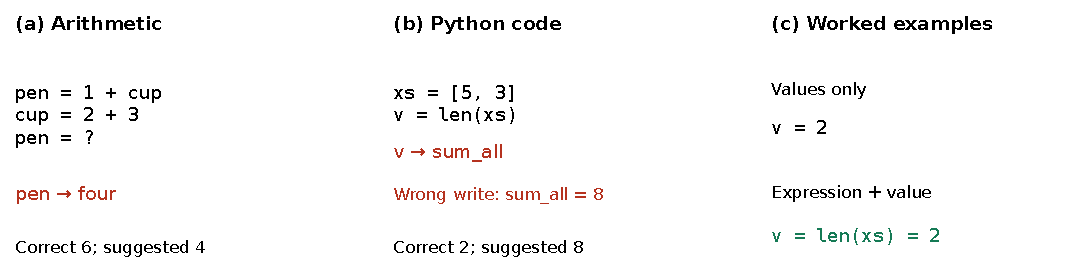
\includegraphics[width=\textwidth]{figures/shared_example.pdf}
\caption{Actual OLMo-2-7B outputs for the same program under two demonstration formats.}
\label{fig:example}
\end{figure*}

\section{Experimental design}
\label{sec:design}

\subsection{Inputs and requested outputs}

Arithmetic problems contain single-digit addition and subtraction, following
\citet{kudo2026faithful}. In the main level, the queried equation precedes the
one needed to evaluate it. For \texttt{pen=1+cup, cup=2+3; pen=?}, the answer is 6.
Code problems contain a short Python function and its input list
(Figure~\ref{fig:example}). Assignments compute length, sum, maximum or minimum,
then integer arithmetic. The main level has three dependent assignments; all
correct assignment values and return values are single digits. Complete task
levels and model panels are in Appendices~\ref{a-app:task} and \ref{c-app:levels}.

Three worked examples precede each test problem. In arithmetic, the model either
writes only the answer or evaluates the equations before answering. In code, it
writes each assignment's value and then the function's return value. We compare
examples showing values alone, such as \texttt{v=2}, with examples showing the
source expression and value, such as \texttt{v=len(xs)=2}. The test program and
\texttt{Trace:} prefix are identical across these formats. Generation is greedy;
three fixed demonstration sets test sensitivity to the examples. Complete prompt
formats are in Appendix~\ref{app:prompts-scoring}.

\subsection{Matched names and output scoring}

Each problem has an ordinary-name twin and a misleading-name version. Inputs,
operations and correct values stay fixed. In arithmetic, renaming \texttt{pen}
to \texttt{four} suggests 4 instead of 6. In code, \texttt{sum\_all} suggests the
sum of a list where the program computes its length. The suggested digit differs
from the correct value and the input digits. This supplies a specific competing
wrong answer whose rate can be compared between the twins.

Table~\ref{tab:scoring} defines the output measurements. The main code error
measurement concerns the first assignment; arithmetic name errors concern the
final answer. We report accuracy alongside these errors to measure whether
outputs become correct. Parse failures remain in all behavioral denominators and
count as incorrect for accuracy. Appendix~\ref{app:prompts-scoring} gives the
parsing rules; Appendix~\ref{app:format-correctness} gives the matched code
correctness cohort.

\begin{table*}[t]
\centering\small
\begin{tabular}{@{}p{.27\textwidth}p{.68\textwidth}@{}}
\toprule
Measurement & What counts \\
\midrule
Intermediate correctness & The written value matches the executed assignment value. \\
Final correctness & The reported answer matches the correct result. \\
Name-suggested error & The target output equals the specific wrong digit suggested by the name. \\
Excess name errors & Misleading-name rate minus ordinary-name rate for that same wrong digit. \\
\bottomrule
\end{tabular}
\caption{Output measurements. Intermediate correctness is reported for the first code assignment.}
\label{tab:scoring}
\end{table*}

\subsection{Measuring internal activity}

A \emph{linear probe} is a separately trained predictor of the correct digit
from one hidden state. In the central code analysis, it reads the state at the
\texttt{=} immediately before an actual wrong value. We also read the end of the
prompt, before the trace starts, on those same error cases. Probe training uses
ordinary-name programs whose computations are disjoint from evaluation.
Layer selection excludes the held-out computation, and the cached prefix must
match the generated prefix through the measurement position. The answer token
is excluded.

A probe measures recoverable information; it does not establish that generation
causally uses that information. The language model generates without the probe.
\emph{Activation patching} instead replaces activity with the ordinary-name twin's
activity and measures the resulting output change. Arithmetic readouts mainly
use supplied correct calculations, with freely generated calculations tested
separately. Probe and patching details are in Appendices~\ref{a-app:recipe},
\ref{c-app:probes} and \ref{c-app:prompt-comparison}.

\subsection{Uncertainty and controls}

Intervals resample computations, keeping both naming conditions and repeated
demonstrations together. A reliable effect requires the same sign across the
three demonstration sets and a 95\% interval excluding zero. A small-effect
claim requires a 90\% interval inside $\pm\NUM{a-eq-delta}$ percentage points.
Intervals are pointwise and condition on fitted layer selectors. Models and
formats remain separate comparisons. Appendix~\ref{c-app:stats} and
Appendix~\ref{app:prompts-scoring} give the sampling and inference details.

\section{Misleading names can change written steps}
\label{sec:behavior}
\label{a-sec:written-controls}

\subsection{Code traces can follow the name's suggested operation}

Misleading names produce substantial wrong intermediate writes when worked
examples list values alone. In length-computing
programs, they add \NUM{c-cell-olmo7-excess}, \NUM{c-cell-llama3-excess} and
\NUM{c-cell-llama8-excess} percentage points of sum writes in OLMo-2-7B,
Llama-3.2-3B and Llama-3.1-8B, respectively. All three checkpoints are
instruction-tuned. These are effects on the first assignment's written value,
not just on the final answer.

The sum is not a common ordinary-name mistake at this step. It accounts for
only \NUM{c-neuerr-sum-lo}--\NUM{c-neuerr-sum-hi}\% of parsed incorrect
ordinary-name writes; maximum values and off-by-one lengths are more common.
On the misleading-name programs, correct first writes fall to
\NUM{j-format-olmo7-values-misleading-first-mean}\%,
\NUM{j-format-llama3-values-misleading-first-mean}\% and
\NUM{j-format-llama8-values-misleading-first-mean}\% (Table~\ref{tab:format-accuracy}).
The matched comparison thus identifies a specific competing calculation that
enters the written trace.

\subsection{Arithmetic provides a comparison with fewer name errors}

Misleading-name effects are generally small when arithmetic calculations are
written. In \NUM{a-eq-cot-equivalent} of \NUM{a-eq-cot-cells} comparisons,
the added-error interval fits within two points of zero. Ten comparisons show a
reliable reduction relative to answer-only output; many answer-only effects are
already small (Appendix~\ref{a-app:round7-paired}). The full behavioral panel and
selected contrasts are in Appendix Table~\ref{a-tab:behavior} and
Figure~\ref{fig:behavior}.

Some output failures remain possible after correct calculations. With an entire
correct generated calculation held fixed, OLMo-2-1B has
\NUM{a-r7-final-olmo-unnamed-mean} added-error points when the final query omits
the variable name. Repeating the name reduces the estimate to
\NUM{a-r7-final-olmo-named-mean} points, while changing ordinary-name accuracy.
These arithmetic comparisons motivate checking outputs even after correct
intermediate work. They provide fewer errors than code for the central readout
test; calibration and competence differences are consolidated in
Section~\ref{sec:scope} and Appendix~\ref{a-app:round7-controls}.

\section{Correct values are recoverable before wrong steps}
\label{sec:readouts}

\begin{figure*}[t]
\centering
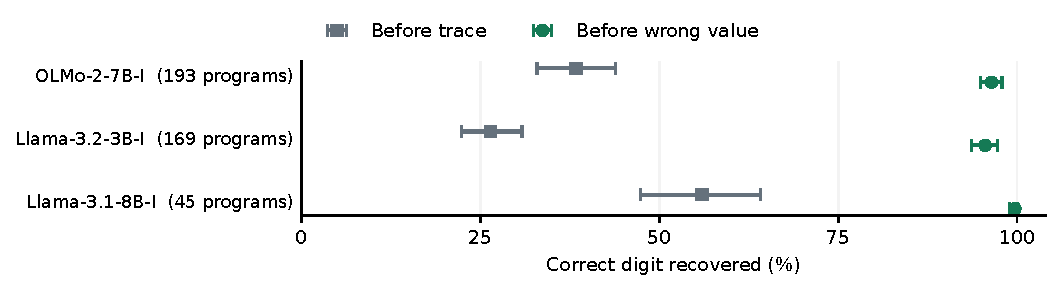
\includegraphics[width=\textwidth]{figures/shared_readouts.pdf}
\caption{Correct-digit recovery on name-suggested wrong writes; counts are unique programs (95\% intervals). I: instruction-tuned.}
\label{fig:readouts}
\end{figure*}

\subsection{Read the state immediately before the observed failure}

On actual sum writes where the code requires length, independently selected
probes recover the correct digit with
\NUM{c-crossfit-min}--\NUM{c-crossfit-max}\% accuracy immediately before the wrong
value is generated (Figure~\ref{fig:readouts}). The figure reports the number of
unique error-producing programs for each model. Multiple demonstration sets
can produce errors on the same program; those repeats remain clustered.

Correct digits are much more readily recovered just before the wrong value than
before the trace starts. Both positions use independent layer selection on the
same error-producing computations. The next written digit is therefore wrong
at a point where the predictor reliably recovers the correct digit.
Appendix~\ref{c-app:prompt-comparison} reports the paired changes and intervals.

The predictors train on \NUM{c-probe-n-train} separate ordinary-name programs,
and select layers without using the held-out computation. The prefix audit
matches the cached state to the actual generation through the \texttt{=} in all
\NUM{c-errorprobe-prefix-n} checked generations. These checks exclude computation
overlap, layer selection on the tested error, and access to the future digit.

\paragraph{Intervention evidence.} Replacing name-token activity with the
ordinary-name twin's activity removes \NUM{c-patch-olmo7-name-best}\% and
\NUM{c-patch-llama3-name-best}\% of name errors in the two code models with
aligned name sites. All-layer pre-value patches remove
\NUM{c-patch-olmo7-pre-all}--\NUM{c-patch-llama8-pre-all}\%; the ordinary-word
control changes at most \NUM{c-patch-llama3-wordctl}\% of correct outputs.
Error removal can yield another wrong value; these whole-state patches test
output sensitivity rather than the decoded digit alone
(Appendices~\ref{c-app:probes} and \ref{a-app:sweeps}).

\section{Showing the operation reduces written errors}
\label{sec:formats}

\subsection{Change the demonstrations, then inspect the same programs}

The strongest practical comparison keeps the program, input, model and
demonstration identities fixed. Replacing \texttt{v=2} examples with
\texttt{v=len(xs)=2} connects the reported value to the source operation.
Added sum writes fall to \NUM{c-cell-olmo7-traceexpr-excess},
\NUM{c-cell-llama3-traceexpr-excess} and \NUM{c-cell-llama8-traceexpr-excess}
points in OLMo-2-7B, Llama-3.2-3B and Llama-3.1-8B, respectively.
Figure~\ref{fig:operation-controls} compares the source expressions with
additional text and numeric elaboration on the same programs.

The improvement includes more correct first writes and final answers, beyond
avoiding the suggested sum (Table~\ref{tab:format-accuracy}).
Ordinary-name correctness remains high;
Appendix~\ref{app:format-correctness} gives both naming conditions and paired
format changes. Each comparison uses 855 paired observations across 285 programs.

\begin{table*}[t]
\centering\small
\begin{tabular}{@{}lrr@{}}
\toprule
Model & \shortstack{Correct first value (\%)\\Values $\to$ expressions} & \shortstack{Correct final answer (\%)\\Values $\to$ expressions} \\
\midrule
OLMo-2-7B-I & \NUM{j-format-olmo7-values-misleading-first-mean} $\to$ \NUM{j-format-olmo7-expression-misleading-first-mean} & \NUM{j-format-olmo7-values-misleading-final-mean} $\to$ \NUM{j-format-olmo7-expression-misleading-final-mean} \\
Llama-3.2-3B-I & \NUM{j-format-llama3-values-misleading-first-mean} $\to$ \NUM{j-format-llama3-expression-misleading-first-mean} & \NUM{j-format-llama3-values-misleading-final-mean} $\to$ \NUM{j-format-llama3-expression-misleading-final-mean} \\
Llama-3.1-8B-I & \NUM{j-format-llama8-values-misleading-first-mean} $\to$ \NUM{j-format-llama8-expression-misleading-first-mean} & \NUM{j-format-llama8-values-misleading-final-mean} $\to$ \NUM{j-format-llama8-expression-misleading-final-mean} \\
\bottomrule
\end{tabular}

\caption{Correct outputs on the same misleading-name programs under both example formats.}
\label{tab:format-accuracy}
\end{table*}

\begin{figure*}[t]
\centering
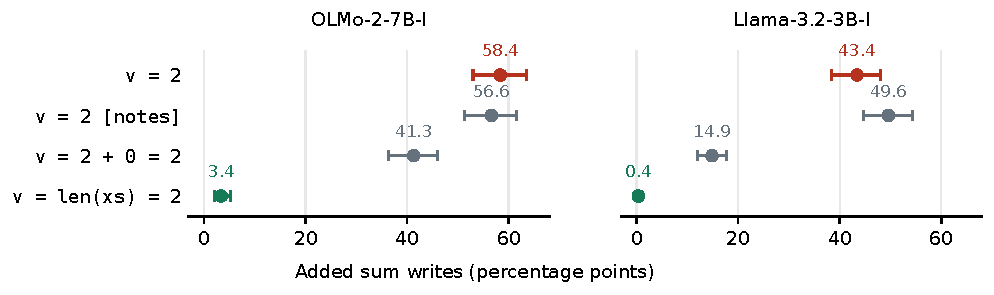
\includegraphics[width=\textwidth]{figures/operation_controls.pdf}
\caption{Demonstration-format controls (95\% intervals). [notes]: matched descriptive text. I: instruction-tuned.}
\label{fig:operation-controls}
\end{figure*}

Matched descriptive text leaves large name effects, while valid numeric
elaboration, such as \texttt{v=2+0=2}, helps partly. Source expressions give the
largest reduction among these controls. Token counts are matched in the
demonstrated outputs, with the test program and trace prefix unchanged. The
benefit therefore depends on what the added text contains. Paired changes and
intervals are in Appendix~\ref{c-app:round5-formats}.

\subsection{The format contrast replicates with fresh names}
\label{sec:replication}

The original code design planned to retain names that evoke their intended
operation in at least 80\% of models, but the runs retained the full name table.
To test the format contrast with independently selected names, we screen
\NUM{c-r6-screen-n} fresh sum-family candidates by their
highest-scoring operation continuation before testing traces. Of these,
\NUM{c-r6-screen-passed} pass the 80\% panel criterion. We freeze the first
\NUM{c-r6-name-n} qualifying names and cross them with
\NUM{c-r6-program-n} new length-computing programs. The computations are absent
from the original training and test data and every demonstration set.

With values-only examples, added sum writes are
\NUM{c-r6-olmo7-trace-mean}, \NUM{c-r6-llama3-trace-mean}
and \NUM{c-r6-llama8-trace-mean}
points in OLMo-2-7B and the two Llama models. Expression-and-value examples reduce
these to \NUM{c-r6-olmo7-expression-mean} points in OLMo and zero observed excess
in both Llamas. The prespecified CodeGemma-7B control has zero observed excess
in both formats. Figure~\ref{fig:fresh-names} shows that the contrast holds across
all three selected names. Intervals cluster repeated demonstrations of each computation;
pooled intervals also cluster names (Appendix~\ref{c-app:round6-identifiers}).
This replication tests the format contrast on new names and programs. The
internal readouts and patches concern the original cohort.

\begin{figure*}[t]
\centering
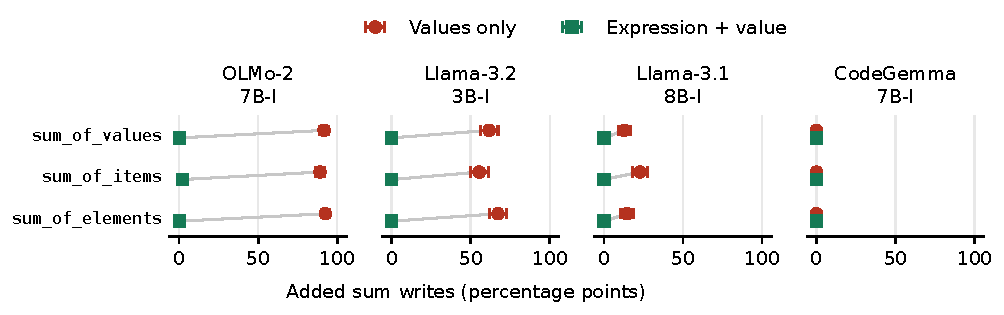
\includegraphics[width=\textwidth]{figures/fresh_names.pdf}
\caption{Fresh names on 200 new length computations (95\% intervals). I: instruction-tuned.}
\label{fig:fresh-names}
\end{figure*}

\section{Scope of the findings}
\label{sec:scope}

\paragraph{Models and formats.} The discrepancy is strongest in three code
checkpoints under values-only demonstrations. Other models and operation
pairings show different effects (Appendix~\ref{c-app:matrix}). Interactive
Python transcripts and values written as code comments also reduce name errors
(Appendix Table~\ref{tab:formats}); source expressions are one effective format.
The reported direct-answer contrasts rename the returned variable, whereas
the central trace comparison renames the first assignment.
Those contrasts do not isolate an effect of requesting a trace.

\paragraph{Arithmetic readouts.} Under supplied correct calculations, arithmetic
probes reproduce the progression of readable values studied by Kudo et al.
Freely generated calculations present a harder transfer test. OLMo's probes
fail the 90\% ordinary-name calibration criterion, and Llama's error cases are
rare. Arithmetic therefore does not establish the same strong error-conditioned
readout result as code. Calibration and correlation details are in
Appendices~\ref{a-app:round6-generated} and \ref{a-app:round5-competence}.

\paragraph{Arithmetic demonstration content.} Repeated names are unnecessary in
the tested competent Llama equation formats. Named and unnamed equations both
reach 99--100\% ordinary-name accuracy and near-zero excess; four role
comparisons pass the held-out competence check. Values-only formats and OLMo's
unnamed equations change competence, preventing an equation-content comparison
at matched accuracy (Appendix~\ref{a-app:round7-controls}).

\paragraph{Scale and natural code.} CodeLlama-34B's maximum-to-sum excess is
\NUM{c-cell34-max-excess} points [\NUM{c-cell34-max-lo}, \NUM{c-cell34-max-hi}];
its interval crosses the two-point small-effect margin. In the
\NUM{c-crux-n}-function CRUXEval check \citep{gu2024cruxeval}, accuracy
contrasts cover zero on the \NUM{c-crux-used} functions that use the renamed
variable downstream. Those conditions request direct answers or prose;
they do not test the synthetic trace or establish equivalence
(Appendix~\ref{c-app:boundaries}).

\section{Related work}

\paragraph{Computation during reasoning.} \citet{kudo2026faithful} track arithmetic
values with probes and activation interventions, finding that answers develop
during the calculation. We retain their controlled arithmetic and probe recipe,
then introduce a name with a competing answer and extend the conflict to programs.
Our code timing comparison concerns the same observed wrong writes before and
during a trace. Work on positional readouts and shortcut solutions also motivates
testing what a readout establishes \citep{liu2026readout,prabhakar2024deciphering}.

\paragraph{Names and misleading wording.} Identifier changes affect code
comprehension and robustness \citep{gao2023cream,le2025names,lam2025codecrash,
le2026obfuscated,orvalho2025mutations}. Our tasks provide an executable correct
value and a distinct value suggested by the name. The matched comparison measures
which incorrect value changes, rather than attributing every accuracy loss to
the same influence. Stroop and cue-conflict studies supply a related experimental
logic \citep{stroop1935,geirhos2019texture,wang2026stroop,hu2026conflict}; the analogy
does not establish a shared human and model mechanism.

\paragraph{Written reasoning and internal information.} Faithfulness studies
show that explanations can omit influences on outputs or react differently to
perturbations \citep{turpin2023unfaithful,lanham2023measuring,chen2025reasoning}.
\citet{orgad2025know} show that internal representations can identify correct
answers among generated candidates even when the model tends to answer
incorrectly. Our contribution measures recovery before an incorrect
\emph{intermediate} write, with the answer token excluded and a controlled name
suggesting a particular competing value. We also test a demonstration-format
change that improves intermediate and final correctness on the same programs.
Probe controls and activation interventions assess recoverability and output
sensitivity separately \citep{hewitt2019control,zhang2024patching}.

\section{Discussion and conclusion}

The central finding is a discrepancy at the point of writing. Correct digits
are recoverable immediately before a model writes conflicting digits suggested
by variable names. Demonstrations showing the producing operation sharply
reduce those errors and increase correct outputs. These observations have three
implications.

\paragraph{Interpreting internal measurements.} Successful decoding establishes
recoverable information, but neither guarantees that the model will write it
nor proves that generation causally uses it. The code error cohorts demonstrate
this distinction directly. More selective interventions are needed to test the
decoded value's role in generation.

\paragraph{Evaluating written reasoning.} Score intermediate values alongside
final answers. Preserve the computation and introduce a name suggesting a
particular competing answer, then report its excess over the ordinary-name
twin together with overall correctness. Repeat across demonstration sets and
formats. This separates a specific misleading-name error from general task
competence and avoids treating a small excess as proof of success.

\paragraph{Designing demonstrations.} What each written step contains matters.
Source-operation examples improve the tested code traces, including on fresh
names and programs. Matched additional text leaves large effects; numeric
elaboration reproduces only part of the benefit. The next test is transfer to
larger programs and natural explanations with adequate ordinary-name accuracy.
The current evidence establishes an effective format change and the gap it
reduces, without identifying a complete causal explanation of that gap.

\section*{Limitations}

\begin{itemize}
\item \textbf{Tasks and formats.} Inputs are synthetic arithmetic and short programs
with single-digit values. The largest code effects use a values-only trace;
interactive Python and comment formats show smaller effects. A
\NUM{c-crux-n}-function CRUXEval check tests direct-answer and prose accuracy, not
the synthetic trace. Its intervals cover zero and do not establish equivalence
within the two-point margin. Models reach 34B, but the arithmetic and code panels
differ in checkpoints and do not cover all model families.
\item \textbf{Readouts and interventions.} The central code probes cover three models.
For length-computing programs, a probe may recover the number of list items or
related input features; it does not identify how that value was computed inside
the model. Arithmetic probes are unreliable on OLMo's freely written calculations,
and the Llama models make too few errors for the same strong test. Patches replace mixed
representations and may produce another wrong answer. Neither the probes nor the
patches identify one mechanism shared across the tasks.
\item \textbf{Selection and competence.} The original code identifiers depart from the
planned meaning gate; the independently screened replication tests new names and
computations. Accuracy changes accompany several arithmetic format controls.
Conditional correct-calculation cohorts do not estimate the effect of making
a calculation correct. Intervals condition on fitted selectors and the tested
demonstrations; related checkpoints and repeated roles are not independent models.
\end{itemize}

\bibliography{refs}
\appendix
\section{Prompts and output scoring}
\label{app:prompts-scoring}

\paragraph{Arithmetic prompts.} The main few-shot prompt concatenates three
same-level ordinary-name demonstration blocks, separated by blank lines, followed
by the test equations and query. Each demonstration contains its equations and
query on one line and its answer or calculation on the next. Answer-only output
has the form \texttt{pen=6}. Calculation output restates equations, substitutes
resolved values and reports each evaluated value in dependency order, ending
with the queried variable. The test prompt ends immediately after its input line
and a newline. Demonstrations reserve a name pool disjoint from test names;
letter-name replication uses letter-name demonstrations. Task levels and
name conditions are in Appendix~\ref{a-app:task}; additional equation and final-query
formats are in Appendix~\ref{a-app:round7-controls}.

\paragraph{Code prompts.} Both main code formats concatenate three ordinary-name
worked examples, separated by blank lines, followed by the test function, its
call and \texttt{Trace:}. There is no additional instruction or interpreter
execution. Each example contains the program and input call, a \texttt{Trace:}
line and an \texttt{Answer:} line. Table~\ref{tab:code-demonstrations} gives the
complete level-5 demonstration set used for Figure~\ref{fig:example}. Assemble
one format by choosing its trace for each example. Both formats then append the
same test program from that figure and the same \texttt{Trace:} prefix. Traces
wrap here for typesetting; each is one line in the prompt. The additional formats
are specified in Appendix~\ref{c-app:formats}.

\begin{table*}[t]
\centering\small
\begin{tabular}{@{}p{.32\textwidth}p{.25\textwidth}p{.37\textwidth}@{}}
\toprule
Program and input & Values-only trace & Expression-and-value trace \\
\midrule
\texttt{def f(xs):}\newline \hspace*{1em}\texttt{u = min(xs)}\newline \hspace*{1em}\texttt{t = u + 1}\newline \hspace*{1em}\texttt{k = t * 2}\newline \hspace*{1em}\texttt{return k}\newline \texttt{f([0,\allowbreak{} 6,\allowbreak{} 5])} & \texttt{u = 0,\allowbreak{} t = 1,\allowbreak{} k = 2}\newline \texttt{Answer: 2} & \texttt{u = min(xs) = 0,\allowbreak{} t = u + 1 = 1,\allowbreak{} k = t * 2 = 2}\newline \texttt{Answer: 2} \\
\addlinespace
\texttt{def f(xs):}\newline \hspace*{1em}\texttt{z = len(xs)}\newline \hspace*{1em}\texttt{r = z * 2}\newline \hspace*{1em}\texttt{k = r - 1}\newline \hspace*{1em}\texttt{return k}\newline \texttt{f([2,\allowbreak{} 4,\allowbreak{} 1])} & \texttt{z = 3,\allowbreak{} r = 6,\allowbreak{} k = 5}\newline \texttt{Answer: 5} & \texttt{z = len(xs) = 3,\allowbreak{} r = z * 2 = 6,\allowbreak{} k = r - 1 = 5}\newline \texttt{Answer: 5} \\
\addlinespace
\texttt{def f(xs):}\newline \hspace*{1em}\texttt{p = len(xs)}\newline \hspace*{1em}\texttt{ww = p + 2}\newline \hspace*{1em}\texttt{u = ww // 2}\newline \hspace*{1em}\texttt{return u}\newline \texttt{f([3,\allowbreak{} 6,\allowbreak{} 0])} & \texttt{p = 3,\allowbreak{} ww = 5,\allowbreak{} u = 2}\newline \texttt{Answer: 2} & \texttt{p = len(xs) = 3,\allowbreak{} ww = p + 2 = 5,\allowbreak{} u = ww // 2 = 2}\newline \texttt{Answer: 2} \\
\addlinespace
\bottomrule
\end{tabular}
\caption{Complete code demonstration set 7; prepend \texttt{Trace:} to each trace.}
\label{tab:code-demonstrations}
\end{table*}


\paragraph{Parsing and denominators.} For code few-shot output, parsing stops at
the first blank line, so an invented subsequent problem cannot supply the answer.
The final answer is the last \texttt{Answer: <integer>} in that block; answer-only
continuations may instead start with the integer directly. A trace value is the
last integer immediately following an equals sign in the target variable's
first assignment clause, before \texttt{Answer:}. This retains the evaluated
value in an expression-and-value trace rather than an operand. A comma followed
by another assignment ends that clause. Interactive transcripts read the integer
following the queried variable; comments read its end-of-line value. Free prose
uses the final \texttt{Answer:} occurrence, or the last integer on the final
nonempty line when that marker is absent.

For arithmetic few-shot output, the answer is the last standalone
\texttt{<queried-name>=<integer>} clause before the first blank line. Free-text
arithmetic uses a queried-name assignment or a final integer fallback. The
reported main arithmetic name-error rate grades this final answer. Code
intermediate correctness grades the first assignment against the program's
executed value; final correctness grades the return value. Parse failures count
as incorrect for accuracy and do not match a name-suggested digit. They remain
in every behavioral denominator. Error-conditioned probes separately use the
observed wrong-write cohort with verified generated prefixes.

\paragraph{Sampling and uncertainty.} Main behavior uses demonstration seeds
7, 11 and 13, with three examples per set and greedy full-vocabulary decoding.
The arithmetic panel contains \NUM{a-n-models} checkpoints and
\NUM{a-n-test-sets} matched sets per task level. The code panel contains
\NUM{c-n-models} instruction-tuned checkpoints, with an additional 34B check,
and 1,000 matched problems per target at levels 3 and 5. The central code cohort
has \NUM{c-probe-n-test} unique length-to-sum computations per set. Checkpoints
and prompts differ between tasks; their results are not pooled.

Resampling retains both names and all demonstration repeats of a computation.
Behavioral reliability requires a consistent sign in all three sets and a 95\%
interval excluding zero. The small-effect criterion uses a 90\% interval within
the prespecified two-point margin. Code timing and matched correctness intervals
use 4,000 draws; the code equivalence audit uses 2,000. Intervals are pointwise,
and probe intervals condition on the fixed independent layer selectors. These
procedures are detailed in Appendices~\ref{c-app:stats},
\ref{c-app:prompt-comparison} and \ref{app:format-correctness}; arithmetic repeated-
computation checks are in Appendix~\ref{a-app:round7-paired}.

\paragraph{Probe fitting and records.} Predictors use three initialization seeds,
0, 1 and 2, and full-batch SGD at learning rate $10^{-3}$ for 10,000 epochs.
Training and evaluation are disjoint in computation, ignoring identifier
spelling. Five-fold layer selection excludes the held-out computation. Cached
prefix checks exclude the future answer token. Optimizer checks, controls,
software versions and data records are in Appendices~\ref{a-app:recipe},
\ref{c-app:round6-probes} and \ref{c-app:reproducibility}.

% Submission appendix: methods and evidence for the reported claims.
\section{Arithmetic task and reproducibility}
\label{a-app:task}

\begin{table}[t]
\centering\small
\resizebox{\columnwidth}{!}{\begin{tabular}{@{}ll@{}}
\toprule
Name & Problem (answer: 6) \\
\midrule
Neutral & \texttt{pen=1 + cup, cup=2 + 3; pen=?} \\
Congruent & \texttt{\textcolor{con}{six}=1 + cup, cup=2 + 3; six=?} \\
Incongruent & \texttt{\textcolor{inc}{four}=1 + cup, cup=2 + 3; four=?} \\
\bottomrule
\end{tabular}}
\caption{Matched names preserve the arithmetic. The misleading digit, 4, occurs nowhere else.}
\label{a-tab:conditions}
\end{table}
A problem contains single-digit variables, addition or subtraction, and a query. The five
levels vary dependency order, depth and the presence of an unused equation
(Table~\ref{a-tab:levels}). Three same-level worked examples precede each test problem.
The evaluated models are \NUM{a-model-list}, plus \NUM{a-n-ladder} derived checkpoints
(Appendix~\ref{a-app:kind}). Demonstrations use ordinary names for every word-name
condition, with a reserved word pool disjoint from test names. Generation is greedy;
only the test variable name changes between matched conditions.

\begin{table}[t]
\centering\small\setlength{\tabcolsep}{4pt}
\resizebox{\columnwidth}{!}{\begin{tabular}{@{}clccc@{}}
\toprule
Level & Problem (neutral names) & Steps & Held & Distr. \\
\midrule
1 & \texttt{pen=1 + cup, cup=2; pen=?} & 1 & 1 & 0 \\
2 & \texttt{pen=2 + 3, cup=1 + pen; cup=?} & 2 & 0 & 0 \\
3 & \texttt{pen=1 + cup, cup=2 + 3; pen=?} & 2 & 1 & 0 \\
4 & \texttt{pen=1 + cup, cup=2 + 3,} & 2 & 1 & 1 \\
  & \texttt{\ \ box=4 + 5; pen=?} & & & \\
5 & \texttt{pen=1 + cup, cup=2 + box,} & 3 & 2 & 0 \\
  & \texttt{\ \ box=1 + 2; pen=?} & & & \\
\bottomrule
\end{tabular}}
\caption{The five levels of \citet{kudo2026faithful}: additions or subtractions needed
(\emph{Steps}), variables unresolved when first read (\emph{Held}), and unused equations
(\emph{Distr.}). At level~1 the intermediate value is stated rather than computed.}
\label{a-tab:levels}
\end{table}

We reimplement \citet{kudo2026faithful}'s task and probe recipe rather than using their code.
The shared choices are single-digit outputs, same-level demonstrations, a 10-way linear
residual-stream classifier, full-batch SGD at $10^{-3}$ for 10,000 epochs, and their
span-by-layer-window patching design. For replication we train on letter names.
The Llama-3.2-3B value-writing positions agree with their Table~3: equation
\NUM{a-replication-eq-v1} for the queried variable and \NUM{a-replication-eq-v2} for the intermediate.
Our additions are the conflicting names, matched baselines, demonstration-set claim rule and
equivalence bound.

Pre-chain probe maxima are \NUM{a-replication-pre-v1} and \NUM{a-replication-pre-v2},
compared with 17.8 and 33.2 in \citet{kudo2026faithful}. The value-writing positions
agree, while the accuracy difference may reflect training details.



\subsection{Tokenizer checks}

\label{a-app:tok}
We test candidate names in five tokenizer contexts and retain words that form one token
without merging with a neighbor. For Llama~3, all ten number words and 95 of 112 neutral
candidates pass. Gemma and OLMo use the same lists; runtime checks confirm equal token lengths
and positions within matched groups. Spaces around binary operators prevent merges such as
\texttt{1-two}. No instance in the reported runs is excluded by the layout check.

\paragraph{Data, compute and software.} Each level has \NUM{a-n-test-sets} matched sets, each
rendered in every condition, and \NUM{a-n-probe-train} separately generated problems for
training probes; every SGD probe is trained with \NUM{a-probe-seeds} seeds. Every run here is
inference and the probes are linear; the three adapter checkpoints of Appendix~\ref{a-app:kind}
were trained in a separate project, and that compute is not counted below. Combined allocation time across the arithmetic and code experiments totals \NUM{a-compute-shared-gpuh} GPU-hours on NVIDIA A30, H100 and H200 cards, an upper bound including idle and shared workers.
The models are from the Llama~3 \citep{grattafiori2024llama3}, Gemma~3 \citep{gemmateam2025gemma3}
and OLMo~2 \citep{olmo2024olmo2,walsh2025olmo2} families, with the reasoning-tuned checkpoint from
\citet{bercovich2025nemotron}, each used under its release licence for research. Models run in
PyTorch \citep{paszke2019pytorch} with Transformers \citep{wolf2020transformers}, and the probes are
trained in PyTorch; the L-BFGS refit of Appendix~\ref{a-app:recipe} uses scikit-learn
\citep{pedregosa2011sklearn}, and the mixed-effects check uses statsmodels
\citep{seabold2010statsmodels}.
Llama checkpoints use the Llama~3.1 or 3.2 Community License, Gemma uses the Gemma Terms
of Use, OLMo uses Apache~2.0, and Nemotron uses the NVIDIA Open Model License.
We use released weights for research inference and do not redistribute them.
Versions are PyTorch~2.11.0 (CUDA~12.9), Transformers~5.14.1, NumPy~2.3.5,
scikit-learn~1.9.1 and SciPy~1.18.0.

\section{Full arithmetic results and controls}
\begin{table*}[t]
\centering\small
\resizebox{\textwidth}{!}{\begin{tabular}{llcrrrr}
\toprule
Model & Regime & Neutral & \multicolumn{2}{c}{number word on the} & \multicolumn{2}{c}{number word on the} \\
& & accuracy & \multicolumn{2}{c}{\emph{queried} variable} & \multicolumn{2}{c}{\emph{intermediate} variable} \\
\cmidrule(lr){4-5}\cmidrule(lr){6-7}
& & (\%) & helps & errors & helps & errors \\
\midrule
Gemma-3-12B-it & CoT & 100\,{\scriptsize[100,100]} & +0.0 & +0.0 & +0.0 & +0.0 \\
Gemma-3-12B-it & direct & 78\,{\scriptsize[76,81]} & -3.2$^{*}$ & -0.2 & -3.7$^{*}$ & +0.4 \\
\addlinespace
Gemma-3-4B-it & CoT & 100\,{\scriptsize[100,100]} & -0.0 & +0.0 & -0.0 & +0.0 \\
Gemma-3-4B-it & direct & 55\,{\scriptsize[48,59]} & +0.2 & +0.9$^{*}$ & +0.6 & +0.3 \\
\addlinespace
Llama-3.1-8B-Instruct & CoT & 100\,{\scriptsize[99,100]} & +0.2 & +0.0 & +0.3 & +0.0 \\
Llama-3.1-8B-Instruct & direct & 52\,{\scriptsize[45,65]} & +1.7 & +0.1 & +5.2$^{*}$ & +0.2 \\
\addlinespace
Llama-3.1-8B & CoT & 95\,{\scriptsize[86,100]} & -1.3 & -0.1 & +3.8 & -0.0 \\
Llama-3.1-8B & direct & 53\,{\scriptsize[41,62]} & +4.8$^{*}$ & +1.2$^{*}$ & +3.8$^{*}$ & -0.0 \\
\addlinespace
Llama-3.2-3B-Instruct & CoT & 100\,{\scriptsize[100,100]} & -0.0 & +0.0 & -0.2 & +0.0 \\
Llama-3.2-3B-Instruct & direct & 44\,{\scriptsize[40,50]} & -1.8$^{*}$ & +0.2 & +0.5 & +0.5 \\
\addlinespace
Llama-3.2-3B & CoT & 98\,{\scriptsize[97,100]} & -1.2 & +0.1 & +0.9 & -0.2$^{*}$ \\
Llama-3.2-3B & direct & 22\,{\scriptsize[13,31]} & +5.4$^{*}$ & +2.8$^{*}$ & +1.1 & +1.8 \\
\addlinespace
OLMo-2-7B-Instruct & CoT & 95\,{\scriptsize[93,97]} & +0.7$^{*}$ & -0.1 & -2.7 & -0.0 \\
OLMo-2-7B-Instruct & direct & 54\,{\scriptsize[50,58]} & +0.6 & -0.2 & +3.8$^{*}$ & -0.4 \\
\bottomrule
\end{tabular}
}
\caption{Arithmetic level 3. Accuracy (\%); name effects (points). *Reliable across demonstration sets.}
\label{a-tab:behavior}
\end{table*}

\begin{table*}[t]
\centering\small
\begin{tabular}{llcrrrr}
\toprule
Model & Regime & Neutral & \multicolumn{2}{c}{number word on the} & \multicolumn{2}{c}{number word on the} \\
& & accuracy & \multicolumn{2}{c}{\emph{queried} variable} & \multicolumn{2}{c}{\emph{intermediate} variable} \\
\cmidrule(lr){4-5}\cmidrule(lr){6-7}
& & (\%) & helps & errors & helps & errors \\
\midrule
OLMo-2-1B-Instruct & CoT & 47\,{\scriptsize[44,51]} & -5.7$^{*}$ & +0.4 & +7.0$^{*}$ & +3.2$^{*}$ \\
OLMo-2-1B-Instruct & direct & 34\,{\scriptsize[30,38]} & -0.0 & +2.7$^{*}$ & +3.0$^{*}$ & -0.2 \\
\bottomrule
\end{tabular}

\caption{The level-3 model below the preregistered 90\% mean neutral-CoT accuracy floor,
excluded from the accuracy-filtered behavioral table. Columns and claim markers follow Table~\ref{a-tab:behavior}.}
\label{a-tab:excluded}
\end{table*}

\subsection{Equivalence and accuracy floor}

\label{a-app:equivalence}
Following preregistration Amendment~3, equivalence requires a 90\% cluster-bootstrap
interval wholly inside the $\pm\NUM{a-eq-delta}$-point margin (two one-sided 5\% tests).
We resample matched sets with their demonstration-seed replicates together, using 4,000
bootstrap draws. Other behavioral intervals remain at 95\%.
For CoT accuracy, \NUM{a-eq-acc-equivalent} of \NUM{a-eq-acc-cells} facilitation and interference
contrasts meet the same equivalence bound. Of the \NUM{a-cot-acc-cells} reliable accuracy
contrasts, \NUM{a-eq-acc-claimable-equivalent} are also equivalent within the margin and
\NUM{a-eq-acc-claimable-outside} are not; a detectable effect can still be small.
The written-value control uses the same matched pairs for its excess estimate and interval;
the exception model's estimate pools all three demonstration sets and clusters on matched set.
\begin{table}[h]
\centering\small
\begin{tabular}{@{}lrrr@{}}
\toprule
Contrast & Cells & Equivalent & Reliable \\
\midrule
CoT name errors & 44 & 43 & 3 \\
CoT accuracy & 88 & 61 & 15 \\
Direct name errors & 44 & 31 & 13 \\
\bottomrule
\end{tabular}

\caption{Equivalence within the two-point margin uses 90\% intervals; reliability uses
95\% intervals excluding zero and the same sign across all three demonstration sets.
Each accuracy cell is one facilitation or interference contrast.}
\end{table}
\begin{table*}[t]
\centering\small
\resizebox{\textwidth}{!}{\begin{tabular}{lclcrrrr}
\toprule
Model & Level & Regime & Neutral & \multicolumn{2}{c}{number word on the} & \multicolumn{2}{c}{number word on the} \\
& & & accuracy & \multicolumn{2}{c}{\emph{queried} variable} & \multicolumn{2}{c}{\emph{intermediate} variable} \\
\cmidrule(lr){5-6}\cmidrule(lr){7-8}
& & & (\%) & helps & errors & helps & errors \\
\midrule
Llama-3.1-8B & 1 & CoT & 99\,{\scriptsize[98,100]} & +0.0 & +0.0 & +0.3 & +0.0 \\
Llama-3.1-8B & 1 & direct & 74\,{\scriptsize[38,99]} & +16.1$^{*}$ & +11.2$^{*}$ & +8.8$^{*}$ & +1.3 \\
\addlinespace
Llama-3.2-3B & 1 & CoT & 97\,{\scriptsize[95,100]} & +1.1 & +0.1 & -2.4 & +0.3 \\
Llama-3.2-3B & 1 & direct & 46\,{\scriptsize[21,93]} & +0.6 & +5.9$^{*}$ & -3.9$^{*}$ & +2.6$^{*}$ \\
\addlinespace
Llama-3.1-8B & 2 & CoT & 100\,{\scriptsize[100,100]} & -0.1 & +0.0 & -0.0 & +0.0 \\
Llama-3.1-8B & 2 & direct & 36\,{\scriptsize[33,37]} & +11.8$^{*}$ & +0.7 & +2.6 & +2.2 \\
\addlinespace
Llama-3.2-3B & 2 & CoT & 94\,{\scriptsize[90,98]} & +3.7 & +0.5$^{*}$ & +1.0$^{*}$ & -0.1 \\
Llama-3.2-3B & 2 & direct & 29\,{\scriptsize[27,30]} & +10.8$^{*}$ & +2.5$^{*}$ & +2.6$^{*}$ & +2.2 \\
\addlinespace
Llama-3.1-8B & 4 & CoT & 88\,{\scriptsize[63,100]} & +1.0 & -0.0 & -2.3 & +0.2 \\
Llama-3.1-8B & 4 & direct & 28\,{\scriptsize[26,31]} & +13.7$^{*}$ & +5.8 & +6.0$^{*}$ & +0.2 \\
\addlinespace
Llama-3.2-3B & 4 & CoT & 64\,{\scriptsize[26,85]} & -10.2$^{*}$ & +0.7 & -2.6$^{*}$ & +0.4 \\
Llama-3.2-3B & 4 & direct & 20\,{\scriptsize[16,23]} & -1.6 & +1.9 & -0.2 & +1.2$^{*}$ \\
\addlinespace
Llama-3.1-8B & 5 & CoT & 65\,{\scriptsize[43,100]} & +1.2 & -0.3 & +0.1 & -0.1 \\
Llama-3.1-8B & 5 & direct & 20\,{\scriptsize[13,26]} & +20.2$^{*}$ & +20.5$^{*}$ & +0.9 & +0.4 \\
\addlinespace
Llama-3.2-3B & 5 & CoT & 69\,{\scriptsize[48,97]} & -1.4 & +0.1 & -2.5 & -0.1 \\
Llama-3.2-3B & 5 & direct & 12\,{\scriptsize[11,12]} & +4.7$^{*}$ & +3.5$^{*}$ & +1.1$^{*}$ & +0.5 \\
\bottomrule
\end{tabular}
}
\caption{Additional task levels for the two Llama models. Columns and claim markers
follow Table~\ref{a-tab:behavior}; level~1 states the intermediate value directly.}
\label{a-tab:levels-appendix}
\end{table*}
\subsection{Naming and written-value controls}

\label{a-app:controls}

\paragraph{Written values.} We split generated chains by whether they state the target's true
value. An observation enters the excess estimate only when its neutral twin falls in the same
split. The estimate and its 95\% interval use those same paired observations. Pooled over
eligible cells, the excess is \NUM{a-vw-excess-wrote} points in \NUM{a-vw-cells-wrote} cells where
the value is stated and \NUM{a-vw-excess-not} in \NUM{a-vw-cells-not} where it is not. The exception
persists in the stated-value split (main text), so this split does not explain its effect.

\paragraph{Identifier-style names.} At level~3, \NUM{a-ident-models} models receive names such as
\texttt{q4} instead of \texttt{four}, under three demonstration sets. Without CoT, queried-variable
excess name errors range from \NUM{a-ident-direct-lure-lo} to \NUM{a-ident-direct-lure-hi} points;
\NUM{a-ident-direct-lure-claim} of \NUM{a-ident-direct-cells} cells are reliable. For number words
on the same models, the range is \NUM{a-word-direct-lure-lo} to \NUM{a-word-direct-lure-hi}, with
\NUM{a-word-direct-lure-claim} of \NUM{a-word-direct-cells} reliable. The numeric name-error effect is
therefore stronger for number words in this comparison; congruent identifier names can still
improve accuracy.

\paragraph{Word-class effects.} With CoT at level~4, a number word on the queried variable costs
Llama-3.2-3B \NUM{a-wordclass-cost-L4} accuracy points whether the name agrees with the value or
not. Those errors restate the wrong equation. This is distinct from answering the digit the
name denotes, which is why the name-suggested value result cannot be read as removal of every naming effect.

\paragraph{Unused variables.} A number word on the level~4 distractor changes accuracy by at
most \NUM{a-irr-acc-delta-max} points. Its no-CoT excess name errors range from \NUM{a-irr-direct-lo} to
\NUM{a-irr-direct-hi}; \NUM{a-irr-direct-claimable} of \NUM{a-irr-direct-cells} cells are reliable.
With CoT, the range is \NUM{a-irr-cot-lo} to \NUM{a-irr-cot-hi}, with
\NUM{a-irr-cot-claimable} of \NUM{a-irr-cot-cells} reliable.

\paragraph{Mixed-effects check.} We compare the paired bootstrap with a mixed logit model,
\texttt{name\_error \textasciitilde{} incongruent + C(seed)}, with a random intercept for
matched set. Each twin's outcome refers to the same name-suggested digit. Both procedures use the same
fixed subsample of \NUM{a-mix-cap} sets per cell. Of \NUM{a-mix-cells} fitted cells,
\NUM{a-mix-agree} agree on whether the interval excludes zero; \NUM{a-mix-unfitted} additional
cells have no outcome variation. The mixed fit supports an effect in \NUM{a-mix-gained} cells
where the bootstrap does not and withdraws support in \NUM{a-mix-lost} cells where it does
(\NUM{a-mix-lost-cells}). Subsampling also removes support from \NUM{a-mix-sub-lost-n} starred
Table~\ref{a-tab:behavior} cell under both procedures (\NUM{a-mix-sub-lost-cells}). The mixed
model uses variational Bayes, so its interval is an approximate posterior interval. We retain
the full-data bootstrap as the primary estimate on the reported percentage-point scale.

\paragraph{Positional-copy control.} Across \NUM{a-copy-n-err} generated CoT name errors over
models, levels and demonstration sets, the final number in the comma-delimited segment before the answer is the
name-suggested value in \NUM{a-copy-lure-frac} of cases and the target's true value in \NUM{a-copy-true-frac}.
A trailing name-suggested value is therefore absent from many errors. This check constrains the positional-copy
explanation of \citet{liu2026readout}, but does not identify what was copied in each case.

\subsection{Derived checkpoints}

\label{a-app:kind}

We compare six checkpoints on the Llama-3.1-8B architecture: pretrained, instruction-tuned,
single-task LoRA, multi-task LoRA, TIES-merged adapters and reasoning-tuned. Adapters are folded
into the weights before evaluation. Shared tokenizers and identical matched problems permit
paired comparisons (Table~\ref{a-tab:kind}). A pretrained/instruct Gemma pair supplies a second
family comparison.

\begin{table*}[t]
\centering\small
\sbox{\appendixtablebox}{\begin{tabular}{@{}llrrr@{}}
\toprule
Tuning & Model & Queried & Intermediate & Acc. \\
\midrule
base & Llama-3.1-8B & +1.20$^{*}$ & -0.02 & 53.4 \\
instruct & \quad + instruct & +0.15 & +0.22 & 52.2 \\
single-task finetune & \quad + task LoRA & +0.05 & +0.23 & 52.2 \\
multi-task finetune & \quad + multi-task LoRA & -0.58$^{*}$ & -0.08 & 46.1 \\
weight merge & \quad + TIES merge & -0.10 & +0.10 & 51.9 \\
reasoning-tuned & Nemotron-Nano-8B & +1.35$^{*}$ & +0.33 & 39.4 \\
\midrule
base & Gemma-3-4B & +0.08 & +0.02 & 60.2 \\
instruct & \quad + instruct & +0.88$^{*}$ & +0.33 & 54.9 \\
\bottomrule
\end{tabular}
}
\ifdim\wd\appendixtablebox>\textwidth
\resizebox{\textwidth}{!}{\usebox{\appendixtablebox}}
\else\usebox{\appendixtablebox}\fi
\caption{Level 3, no CoT, name errors above the matched twin's rate, mean over three
demonstration sets. \emph{Acc.} is neutral accuracy. $^{*}$ as in Table~\ref{a-tab:behavior}.
The bottom block repeats the pretrained-to-instruct step in a second family, Gemma-3-4B.}
\label{a-tab:kind}
\end{table*}

Task accuracy complicates interpretation. The multi-task model's reliable negative excess
(\NUM{a-kind-ftm-v1}) accompanies lower neutral accuracy (\NUM{a-kind-ftm-acc}\%, versus
\NUM{a-kind-it-acc}\%). The reasoning-tuned checkpoint has the lowest accuracy
(\NUM{a-kind-reas-acc}\%). It also requires a system instruction to enable long-form reasoning;
our raw-completion prompts leave that mode off. The result concerns the checkpoint under this
prompt, not reasoning mode in deployment.
Across these checkpoints, CoT excess name errors are at most \NUM{a-kind-cot-max} points
in magnitude.

\subsection{Values without equations}

\label{a-app:simple}

Our chain restates each equation before substituting into it, as
\citeauthor{kudo2026faithful}'s does. Their Tables~5--6 also report a format that writes only the
sub-results, \texttt{cup=5, pen=6}. We test this format
at level 3 with three demonstration sets. Two predictions were registered for both Llama models: that
the excess name errors at the intermediate's value step would exceed the \NUM{a-eq-delta}-point
margin, and that the value would still be decodable there (probe accuracy at least 0.85), making
any failure one of readout.

Both predictions fail as registered. Llama-3.1-8B writes the name-suggested value at the intermediate's value
step \NUM{a-simple-l8b-v2} points above its twin, inside the margin. Llama-3.2-3B is at
\NUM{a-simple-l3b-v2}, which passes our claim rule, but across the three demonstration sets that
is \NUM{a-simple-l3b-v2-seeds}, so one set carries most of it. More informative is what the probes say. At
the step that writes the value, the true value is decodable at \NUM{a-simpleprobe-l8b-simple-v1}
and \NUM{a-simpleprobe-l8b-simple-v2} for Llama-3.1-8B and at
\NUM{a-simpleprobe-l3b-simple-v1} and \NUM{a-simpleprobe-l3b-simple-v2} for Llama-3.2-3B, against
\NUM{a-simpleprobe-l8b-cot-v1} and \NUM{a-simpleprobe-l8b-cot-v2} for the same model under the full
chain. Neutral accuracy falls with it, to \NUM{a-simple-l8b-acc}\% and \NUM{a-simple-l3b-acc}\%.

Removing the equations lowers both accuracy and true-value probe readouts. It therefore fails to isolate a readout error while preserving those measures.

\section{Probe and patching controls}
\label{a-app:sweeps}
\label{a-app:figs}

% Generated by scripts/66_figure_dump.py: explicit submission selection.
\begin{figure*}[t]
\centering
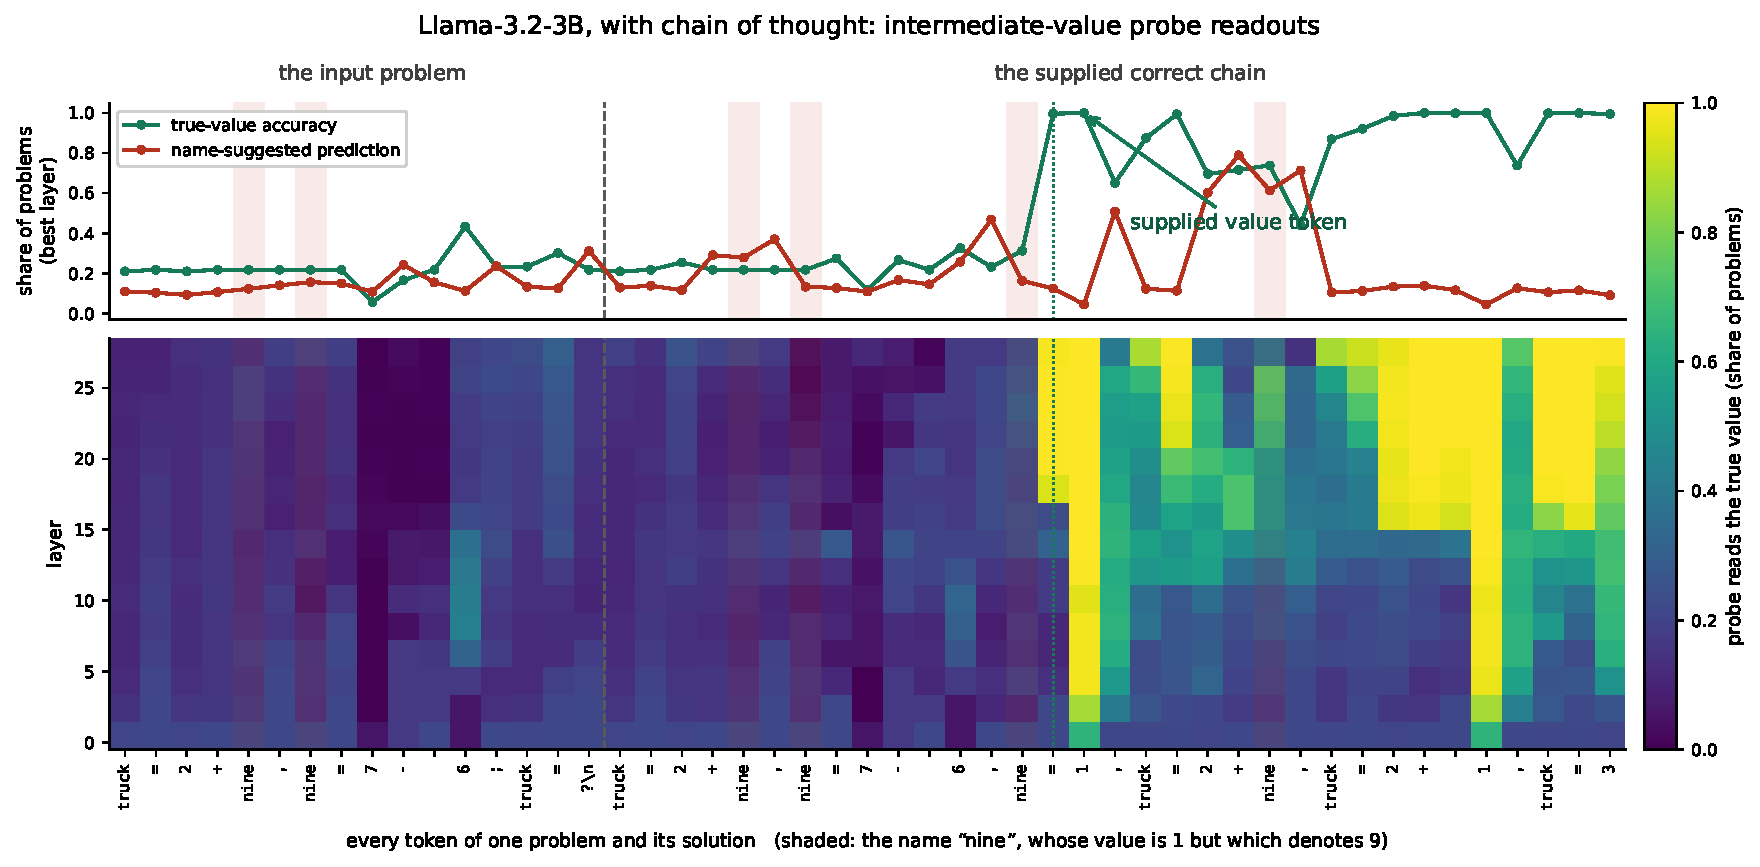
\includegraphics[width=\textwidth]{figures/a_fig2_tokens_llama32-3b_L3_cot_v2.pdf}
\caption{Llama-3.2-3B intermediate-value readouts under supplied correct calculations. Rates pool problems; tokens illustrate one example.}\label{a-fig:heat}
\end{figure*}

\begin{figure*}[t]
\centering
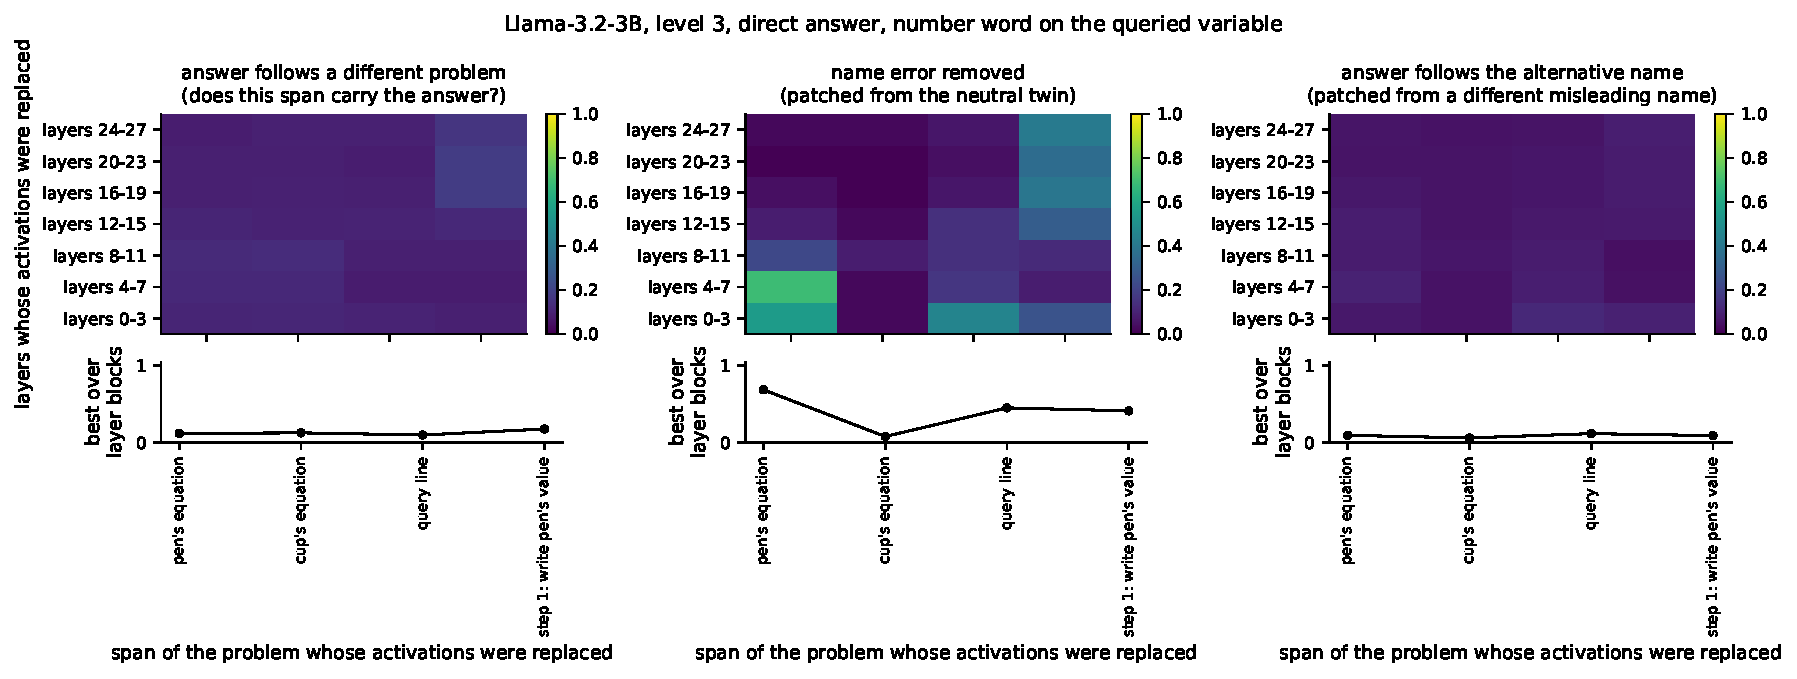
\includegraphics[width=\textwidth]{figures/a_kudo_fig5_llama32-3b_L3_direct_v1.pdf}
\caption{Llama-3.2-3B answer-only patches in four-layer windows. Bottom: maximum over windows.}\label{a-fig:grid}
\end{figure*}


Probes predict the true digit, the name-suggested digit and their probability margin.
The name-identity control assigns a fixed random digit to each name; selectivity subtracts
its accuracy from true-value accuracy. Layers in the supplied-calculation analysis are
selected by neutral selectivity, averaged over three probe seeds.
P1 is the name token, P2 the end of its defining equation, P3 the query,
P4 the position before its value is written, and P5 the position before the final answer.
P1 is a reference, and P3 can reveal name identity rather than a computed value.
Figure~\ref{a-fig:heat} gives the token and layer sweep supporting the main readout analysis.

Patches replace residual-stream activations at matched name-token positions, at individual
layers or across all layers. The neutral-twin source tests removal of the name error;
a different ordinary name tests damage to correct answers; an alternative misleading
name tests specificity. The span sweep instead replaces an equation, the query or the
value-writing segment in four-layer windows. Figure~\ref{a-fig:grid} supports the early-layer
localization. Table~\ref{a-tab:patching-controls} gives the answer-only control rates
and denominators for both Llama models.
OLMo's supplied-calculation controls are reported in Table~\ref{a-tab:exception-patching}.
We also reverse the main contrast, transplanting misleading-name states into the
ordinary-name twin. OLMo's largest injection rate across layers and both variables is
\NUM{a-exc-inject} at layer \NUM{a-exc-inject-layer}; word-control damage there is
\NUM{a-exc-ctlword}. The injection itself damages \NUM{a-exc-inject-damage} of correct
answers. This selected maximum is descriptive.

\begin{table*}[t]
\centering\small
\resizebox{\textwidth}{!}{\begin{tabular}{@{}llrrrrrr@{}}
\toprule
Model & Variable & Pairs & Name errors & Correct & Neutral & Alternative & Word damage \\
\midrule
Llama-3.2-3B & queried & 2000 & 172 & 272 & 51.7 & 34.9 & 22.4 \\
Llama-3.1-8B & intermediate & 2000 & 72 & 838 & 30.6 & 30.6 & 8.5 \\
\bottomrule
\end{tabular}
}
\caption{All-layer answer-only patches, demonstration set 7. Neutral and alternative:
percentage of baseline name errors removed. Word damage: percentage of correct
ordinary-name answers changed; \emph{Correct} gives that denominator.}
\label{a-tab:patching-controls}
\end{table*}

\paragraph{Instance-level association.} Within each model, level, regime, variable and
position, we regress name errors on the probe margin, $\log p_{\mathrm{true}}-\log p_{\mathrm{name}}$,
where $p_{\mathrm{name}}$ is the probe probability of the name-suggested value,
with standard errors clustered on matched set. The layer is selected by neutral accuracy.
Of \NUM{a-link-fits} fits, \NUM{a-link-sig} have $p<.05$: \NUM{a-link-neg} coefficients are negative
and \NUM{a-link-pos} positive. The direction is not consistent, and \NUM{a-link-pos-topmodel-n}
positive results come from the model supplying most fits. This leaves the instance-level
association unresolved. The model-level pattern is also sensitive to panel composition
(Appendix~\ref{a-app:round5-competence}).

\subsection{Probe recipe and patching scope}

\label{a-app:recipe}

We check two implementation choices inherited from \citet{kudo2026faithful}: the probe optimizer and the name occurrences included in a patch.

\paragraph{Recipe.} We refit the level-3 probes for Llama-3.2-3B with L-BFGS, and with SGD on
standardized inputs, against the reported recipe.

\begin{table*}[t]
\centering\small
\sbox{\appendixtablebox}{\begin{tabular}{@{}llrrr@{}}
\toprule
Position & Variable & SGD (reported) & L-BFGS & standardized \\
\midrule
defining equation & queried & 0.184 & 0.190 & 0.183 \\
defining equation & intermediate & 0.496 & 0.422 & 0.420 \\
query & queried & 0.183 & 0.316 & 0.280 \\
query & intermediate & 0.271 & 0.366 & 0.393 \\
value step & queried & 1.000 & 1.000 & 1.000 \\
value step & intermediate & 0.982 & 0.962 & 0.972 \\
answer & queried & 1.000 & 1.000 & 1.000 \\
\bottomrule
\end{tabular}
}
\ifdim\wd\appendixtablebox>\textwidth
\resizebox{\textwidth}{!}{\usebox{\appendixtablebox}}
\else\usebox{\appendixtablebox}\fi
\caption{Best-layer true-value accuracy on neutral problems under three probe recipes
(proportions from 0 to 1).}
\label{a-tab:recipe}
\end{table*}

All three recipes give the same qualitative result: the value is decodable where the chain writes it
(\NUM{a-e17-value-lo}--\NUM{a-e17-value-hi}) and not at the end of its defining equation
(\NUM{a-e17-end-lo}--\NUM{a-e17-end-hi}). The query position moves, from \NUM{a-e17-sgd-query-v2}
under the reported recipe to \NUM{a-e17-std-query-v2} under standardization, within a range of
\NUM{a-e17-query-lo}--\NUM{a-e17-query-hi} over recipes and variables. We already report that
position as the presence of the name rather than a decoded value, because its control task
scores \NUM{a-p3-ctl}, so this variation does not change the interpretation of that position.

\paragraph{Scope.} Patching every occurrence of the name includes the copy the model writes in
its own output. In the direct regime, restricting the patch to the name's occurrences in the prompt leaves the
intermediate variable essentially unchanged, since its name never appears in the answer: removal is
\NUM{a-e18-v2-all-removed}\% at layers~\NUM{a-e18-v2-all-best} under both scopes. For the queried
variable the best windows remove similar shares (\NUM{a-e18-v1-prompt-removed}\% at
layers~\NUM{a-e18-v1-prompt-best} prompt-only, against \NUM{a-e18-v1-all-removed}\% at
layers~\NUM{a-e18-v1-all-best}), the prompt-only patch removes less in the later windows, and the
two disagree most in the first window, where the prompt-only patch removes
\NUM{a-e18-v1-prompt-w03}\% and damages \NUM{a-e18-v1-prompt-w03damage}\% of correct answers. That
is mechanical: the queried variable's name also sits at the position we read, so patching its
prompt copies alone leaves the model reading a name whose early representation no longer
matches. The localization we report does not depend on the choice.

\IfFileExists{tables/a_exception_patching.tex}{%
\begin{table*}[t]
\centering\small
\resizebox{\textwidth}{!}{\begin{tabular}{@{}llrrrrr@{}}
\toprule
Target & Read & Errors & Neutral removed & Word dmg. & Alt. removed & Alt. followed \\
\midrule
v1 & value & 0 & -- & 1.6 & -- & 0.0 \\
v1 & answer & 0 & -- & 1.6 & -- & 0.0 \\
v2 & value & 28 & 92.9 & 7.3 & 82.1 & 4.0 \\
v2 & answer & 3 & 100.0 & 0.8 & 100.0 & 0.6 \\
\bottomrule
\end{tabular}
}
\caption{OLMo-2-1B-Instruct, supplied correct calculations, \NUM{a-exc-controls-n} matched
pairs per target. All-layer rates (\%): neutral/alternative name-error removal, word-control
damage to correct predictions, and predictions following the alternative digit.
Roles v1/v2: queried/intermediate; --: undefined.}
\label{a-tab:exception-patching}
\end{table*}
}{}
% Generated from validated reviewer follow-up JSON.
\section{Task competence and value readouts}
\label{a-app:round5-competence}
Table~\ref{a-tab:round5-competence} compares both variables for 9 models. Layers are selected by neutral selectivity, averaging three probe seeds. Task accuracy and paired excess name errors pool demonstration sets 7, 11 and 13; probes use set 7. The within-model difference holds overall task accuracy fixed but does not isolate a causal effect of the readout.
We average the two variable readouts within each model before computing descriptive correlations. Table~\ref{a-tab:round5-correlation} repeats them after omitting each model. Roles are not independent observations. With this small, heterogeneous panel, correlations cannot distinguish overall competence from the role of decodable information.
\begin{table*}[t]
\centering\small
\sbox{\roundfivebox}{\begin{tabular}{@{}llrrrrrr@{}}
\toprule
Model & Role & Layer & Task & Neutral & Name ID & Misleading & Excess \\
\midrule
Gemma-3-12B-I & v1 & 40 & 100.0 & 100.0 & 13.1 & 100.0 & 0.0 \\
Gemma-3-12B-I & v2 & 42 & 100.0 & 100.0 & 11.9 & 100.0 & 0.0 \\
Gemma-3-4B & v1 & 25 & 100.0 & 100.0 & 10.0 & 100.0 & 0.0 \\
Gemma-3-4B & v2 & 28 & 100.0 & 99.8 & 12.4 & 100.0 & 0.0 \\
Gemma-3-4B-I & v1 & 29 & 100.0 & 100.0 & 7.4 & 99.9 & 0.0 \\
Gemma-3-4B-I & v2 & 28 & 100.0 & 99.8 & 10.0 & 99.9 & 0.0 \\
Llama-3.1-8B & v1 & 20 & 95.2 & 100.0 & 20.5 & 100.0 & -0.1 \\
Llama-3.1-8B & v2 & 22 & 95.2 & 99.4 & 24.9 & 99.2 & -0.0 \\
Llama-3.1-8B-I & v1 & 20 & 99.7 & 100.0 & 21.0 & 100.0 & 0.0 \\
Llama-3.1-8B-I & v2 & 20 & 99.7 & 100.0 & 25.7 & 100.0 & 0.0 \\
Llama-3.2-3B & v1 & 19 & 98.3 & 99.9 & 22.7 & 100.0 & 0.1 \\
Llama-3.2-3B & v2 & 21 & 98.3 & 97.6 & 31.5 & 99.6 & -0.2 \\
Llama-3.2-3B-I & v1 & 18 & 100.0 & 99.9 & 26.3 & 100.0 & 0.0 \\
Llama-3.2-3B-I & v2 & 19 & 100.0 & 99.9 & 29.5 & 99.9 & 0.0 \\
OLMo-2-1B & v1 & 14 & 47.2 & 99.7 & 48.9 & 100.0 & 0.4 \\
OLMo-2-1B & v2 & 0 & 47.2 & 21.8 & 15.0 & 21.8 & 3.2 \\
OLMo-2-7B & v1 & 22 & 95.3 & 100.0 & 37.7 & 100.0 & -0.1 \\
OLMo-2-7B & v2 & 26 & 95.3 & 99.4 & 47.5 & 97.6 & -0.0 \\
\bottomrule
\end{tabular}}
\ifdim\wd\roundfivebox>\textwidth\resizebox{\textwidth}{!}{\usebox{\roundfivebox}}\else\usebox{\roundfivebox}\fi
\caption{Task and true-digit probe accuracies (\%), name-identity control accuracy (\%), and excess name errors (points). Roles v1/v2 are queried/intermediate. Selectivity is neutral minus name-ID accuracy. Below-floor models remain descriptive.}
\label{a-tab:round5-competence}
\end{table*}
\begin{table*}[t]
\centering\small
\sbox{\roundfivebox}{\begin{tabular}{@{}lrrr@{}}
\toprule
Omitted model & Task--excess & Probe--excess & Task--probe \\
\midrule
All models & -0.99 & -1.00 & +1.00 \\
Gemma-3-12B-I & -0.99 & -1.00 & +1.00 \\
Gemma-3-4B & -0.99 & -1.00 & +1.00 \\
Gemma-3-4B-I & -0.99 & -1.00 & +1.00 \\
Llama-3.1-8B & -0.99 & -1.00 & +1.00 \\
Llama-3.1-8B-I & -0.99 & -1.00 & +1.00 \\
Llama-3.2-3B & -0.99 & -1.00 & +1.00 \\
Llama-3.2-3B-I & -0.99 & -1.00 & +1.00 \\
OLMo-2-1B & +0.98 & +0.78 & +0.85 \\
OLMo-2-7B & -0.99 & -1.00 & +1.00 \\
\bottomrule
\end{tabular}}
\ifdim\wd\roundfivebox>\textwidth\resizebox{\textwidth}{!}{\usebox{\roundfivebox}}\else\usebox{\roundfivebox}\fi
\caption{Descriptive Pearson correlations of model means; Spearman values and within-model variable differences are in the saved summary. No significance or causal claim is based on these coefficients.}
\label{a-tab:round5-correlation}
\end{table*}
\section{Gold-trained transfer to generated chains}
\label{a-app:round5-generated}
We read the state before the first numeric assignment to the target in each saved generated chain. Expression operands are not counted as completed value writes; tokens that include any part of the supplied value are excluded. A fixed sample of 200 matched sets is selected by a hash independent of outcomes, shared across models, variables and demonstration sets. All additional chains with name errors and their neutral twins are evaluated separately.
Neutral gold-chain probes use 10,000 separate training problems, three probe seeds and the original neutral-selectivity layer. Table~\ref{a-tab:round5-generated} tests transfer to held-out neutral generated chains. A high-accuracy interpretation requires at least 90\% neutral calibration in that demonstration set. Cases below that threshold yield descriptive readouts only. The augmentation is selected by observed errors and cannot estimate their population rate. Appendix~\ref{a-app:round6-generated} separately trains probes on generated neutral chains and tests the same held-out prefixes.
Llama-3.2-3B meets the neutral transfer threshold in 6 of 6 cells, with calibration accuracy from 97.2 to 100.0\%.
OLMo-2-1B meets the neutral transfer threshold in 0 of 6 cells, with calibration accuracy from 19.4 to 62.2\%.
Name-error cases in the competent model are few; error-conditioned readouts cannot establish a general mechanism from that subset. Failed neutral calibration prevents a strong generated-chain interpretation for the exception model.
\begin{table*}[t]
\centering\small
\sbox{\roundfivebox}{\begin{tabular}{@{}lrrllrr@{}}
\toprule
Model & Set & Role & Neutral coverage & Calibration (\%) & Sample errors & Extra errors \\
\midrule
OLMo-2-1B & 7 & v1 & 194/200 & 62.2 [55.2, 68.7] & 8 & 69 \\
OLMo-2-1B & 7 & v2 & 186/200 & 19.4 [14.0, 25.3] & 11 & 82 \\
OLMo-2-1B & 11 & v1 & 187/200 & 55.3 [48.3, 62.6] & 7 & 59 \\
OLMo-2-1B & 11 & v2 & 129/200 & 21.7 [14.7, 28.7] & 2 & 21 \\
OLMo-2-1B & 13 & v1 & 193/200 & 52.7 [45.6, 59.8] & 17 & 159 \\
OLMo-2-1B & 13 & v2 & 124/200 & 24.2 [16.9, 32.3] & 1 & 30 \\
Llama-3.2-3B & 7 & v1 & 200/200 & 98.0 [96.0, 99.5] & 1 & 8 \\
Llama-3.2-3B & 7 & v2 & 200/200 & 97.2 [94.8, 99.0] & 0 & 0 \\
Llama-3.2-3B & 11 & v1 & 199/200 & 100.0 [100.0, 100.0] & 0 & 0 \\
Llama-3.2-3B & 11 & v2 & 200/200 & 100.0 [100.0, 100.0] & 0 & 0 \\
Llama-3.2-3B & 13 & v1 & 199/200 & 99.5 [98.5, 100.0] & 0 & 5 \\
Llama-3.2-3B & 13 & v2 & 200/200 & 99.5 [98.5, 100.0] & 0 & 0 \\
\bottomrule
\end{tabular}}
\ifdim\wd\roundfivebox>\textwidth\resizebox{\textwidth}{!}{\usebox{\roundfivebox}}\else\usebox{\roundfivebox}\fi
\caption{Gold-trained probe accuracy on neutral generated chains [95\% interval], and eligible name-error counts. Extra cases exclude the fixed sample. Roles v1/v2 are queried/intermediate. Calibration is required before interpreting error readouts.}
\label{a-tab:round5-generated}
\end{table*}

% Generated from validated round-six summary.
\section{Training probes on generated neutral chains}
\label{a-app:round6-generated}
Gold-trained probe transfer (Appendix~\ref{a-app:round5-generated}) may fail because the states along generated chains differ from those along the supplied correct chain. We therefore train on freely generated neutral chains from \NUM{a-r6-source-train_n} source problems and select layers on \NUM{a-r6-source-validation_n} separate validation problems. Canonical equations partition the source pool, keeping renamed versions of a computation together. The training and validation pools contain \NUM{a-r6-source-train_keys} and \NUM{a-r6-source-validation_keys} computations; both exclude all test and demonstration computations. These counts distinguish independent computations from repeated name renderings.
Generation is greedy with demonstration set 7 and a 128-token limit. The probe sees the hidden state before the target variable's first numeric assignment, with every token boundary checked to exclude the value digit. Missing or unsafe boundaries are excluded and counted. We retain all usable neutral chains regardless of whether the model writes the correct value, using the executed true value as the training label. Three probe seeds use the original full-batch SGD recipe (learning rate 0.001, 10,000 epochs). States are stored in float32 and nonfinite states or fitted weights are rejected. Layers are searched at stride two, including the final layer, and chosen only by mean validation accuracy with the lowest-layer tie break. The name-identity control is trained separately and does not select layers.
Table~\ref{a-tab:round6-selection} reports the usable source counts and selected layers. Evaluation uses exactly the earlier fixed 200-set sample and separately reported additional name-error cases under demonstration sets 7, 11 and 13. Table~\ref{a-tab:round6-calibration} gives held-out neutral calibration and boundary coverage. Intervals use 4,000 canonical-computation bootstrap draws, keeping repeated names together. The 90\% calibration threshold applies to the point estimate, not the lower interval endpoint.
Llama passes all six calibration cells; OLMo passes none. Table~\ref{a-tab:round6-errors} retains error readouts with their denominators. OLMo's readouts remain descriptive. Llama has only one name-error case in the primary sample and thirteen additional observed writes; these rare, selected cases cannot establish a general mechanism.
\begin{table*}[t]
\centering\small
\sbox{\roundsixbox}{\begin{tabular}{@{}llrrrrr@{}}
\toprule
Model & Role & Train $n$ & Validation $n$ & Layer & Validation (\%) & Name ID (\%) \\
\midrule
OLMo-2-1B-I & v1 & 1924 & 390 & 14 & 47.9 & 41.6 \\
OLMo-2-1B-I & v2 & 1877 & 376 & 16 & 87.8 & 86.6 \\
Llama-3.2-3B & v1 & 1994 & 398 & 22 & 97.5 & 26.8 \\
Llama-3.2-3B & v2 & 2000 & 400 & 20 & 99.2 & 28.6 \\
\bottomrule
\end{tabular}}
\ifdim\wd\roundsixbox>\textwidth\resizebox{\textwidth}{!}{\usebox{\roundsixbox}}\else\usebox{\roundsixbox}\fi
\caption{Usable generated-boundary counts and validation-selected layers. Roles v1/v2 are queried/intermediate. Source cohorts are computation-disjoint; validation scores are not test estimates.}
\label{a-tab:round6-selection}
\end{table*}
\begin{table*}[t]
\centering\small
\sbox{\roundsixbox}{\begin{tabular}{@{}llrlllc@{}}
\toprule
Model & Role & Set & Neutral coverage & Calibration (\%) & Name ID (\%) & Pass \\
\midrule
OLMo-2-1B-I & v1 & 7 & 194/200 & 61.3 [54.1, 68.6] & 37.3 [31.2, 43.4] & no \\
OLMo-2-1B-I & v1 & 11 & 187/200 & 52.8 [45.1, 60.3] & 32.4 [26.6, 38.5] & no \\
OLMo-2-1B-I & v1 & 13 & 193/200 & 50.3 [43.0, 57.4] & 35.2 [29.1, 41.6] & no \\
OLMo-2-1B-I & v2 & 7 & 186/200 & 78.0 [71.5, 83.9] & 81.9 [76.9, 86.7] & no \\
OLMo-2-1B-I & v2 & 11 & 129/200 & 80.1 [72.8, 86.8] & 56.6 [49.6, 63.3] & no \\
OLMo-2-1B-I & v2 & 13 & 124/200 & 71.8 [64.2, 78.4] & 46.8 [37.8, 55.6] & no \\
Llama-3.2-3B & v1 & 7 & 200/200 & 98.5 [96.7, 100.0] & 18.5 [13.8, 23.7] & yes \\
Llama-3.2-3B & v1 & 11 & 199/200 & 100.0 [100.0, 100.0] & 13.9 [9.5, 18.5] & yes \\
Llama-3.2-3B & v1 & 13 & 199/200 & 97.2 [94.2, 99.5] & 16.9 [12.3, 21.8] & yes \\
Llama-3.2-3B & v2 & 7 & 200/200 & 96.3 [93.6, 98.6] & 28.8 [22.7, 35.0] & yes \\
Llama-3.2-3B & v2 & 11 & 200/200 & 100.0 [100.0, 100.0] & 17.2 [12.4, 22.1] & yes \\
Llama-3.2-3B & v2 & 13 & 200/200 & 97.7 [95.5, 99.3] & 17.8 [13.3, 22.8] & yes \\
\bottomrule
\end{tabular}}
\ifdim\wd\roundsixbox>\textwidth\resizebox{\textwidth}{!}{\usebox{\roundsixbox}}\else\usebox{\roundsixbox}\fi
\caption{Held-out primary neutral generated chains. Coverage counts valid pre-value boundaries over all primary neutral rows. Accuracy intervals are 95\% canonical-computation bootstrap intervals; pass means the calibration point estimate meets 90\%.}
\label{a-tab:round6-calibration}
\end{table*}
\begin{table*}[t]
\centering\small
\sbox{\roundsixbox}{\begin{tabular}{@{}llrrlrl@{}}
\toprule
Model & Role & Set & Sample $n$ & Sample accuracy & Extra $n$ & Extra accuracy \\
\midrule
OLMo-2-1B-I & v1 & 7 & 8 & 4.2 [0.0, 12.5] & 69 & 2.9 [0.0, 7.0] \\
OLMo-2-1B-I & v1 & 11 & 7 & 19.0 [0.0, 38.1] & 59 & 10.7 [4.2, 18.8] \\
OLMo-2-1B-I & v1 & 13 & 17 & 21.6 [7.8, 39.2] & 159 & 13.6 [8.6, 19.4] \\
OLMo-2-1B-I & v2 & 7 & 11 & 33.3 [15.2, 51.5] & 82 & 18.7 [11.4, 27.2] \\
OLMo-2-1B-I & v2 & 11 & 2 & 0.0 [0.0, 0.0] & 21 & 17.5 [3.3, 31.8] \\
OLMo-2-1B-I & v2 & 13 & 1 & 0.0 [0.0, 0.0] & 30 & 25.6 [13.7, 39.1] \\
Llama-3.2-3B & v1 & 7 & 1 & 0.0 [0.0, 0.0] & 8 & 12.5 [0.0, 42.9] \\
Llama-3.2-3B & v1 & 11 & 0 & -- & 0 & -- \\
Llama-3.2-3B & v1 & 13 & 0 & -- & 5 & 0.0 [0.0, 0.0] \\
Llama-3.2-3B & v2 & 7 & 0 & -- & 0 & -- \\
Llama-3.2-3B & v2 & 11 & 0 & -- & 0 & -- \\
Llama-3.2-3B & v2 & 13 & 0 & -- & 0 & -- \\
\bottomrule
\end{tabular}}
\ifdim\wd\roundsixbox>\textwidth\resizebox{\textwidth}{!}{\usebox{\roundsixbox}}\else\usebox{\roundsixbox}\fi
\caption{True-digit accuracy (\%) [95\% interval] on actual name errors, with the fixed sample and additional error-selected cases separated. Extra cases exclude the primary sample. Dashes denote empty strata. OLMo fails neutral calibration, so its readouts are descriptive.}
\label{a-tab:round6-errors}
\end{table*}

% Generated by scripts/88_round7_tables.py from validated paired outputs.
\section{Paired change from answer-only to written calculations}
\label{a-app:round7-paired}
We compare prompting conditions on exactly the same matched sets and demonstration seeds used in the 44 name-error equivalence cells. Each observation subtracts the ordinary-name rate from the misleading-name rate, then subtracts the answer-only contrast from the CoT contrast. Negative changes indicate fewer added name-suggested answers. We bootstrap matched sets, keeping all three demonstration repeats together (4,000 draws). Reliable reductions require a negative change in every demonstration set and a 95\% interval below zero. The panel is descriptive across related checkpoints; its cells are not independent model replications.
Of the 44 paired changes, 10 meet that rule; 19 have intervals below zero. A sensitivity bootstrap that also clusters repeated arithmetic computations yields 10 reliable reductions. Intervals are pointwise; the count is not a multiplicity-corrected family-wide test. Before writing calculations, 31 cells already meet the two-point equivalence bound, compared with 43 afterward. Thus the equivalence count is not a count of significant improvements. Accuracy gains accompany many reductions and do not identify an effect independent of arithmetic competence.
\begin{table*}[t]
\centering\small
\sbox{\roundsevenbox}{\begin{tabular}{@{}llrrrr@{}}
\toprule
Model & Level/role & Answer-only & CoT & Paired change [95\% interval] & Accuracy gain \\
\midrule
Llama-3.2-3B & L1/v1 & +5.90 & +0.12 & -5.78 [-6.55, -5.02]$^{*}$ & +50.7 \\
Llama-3.2-3B & L1/v2 & +2.62 & +0.30 & -2.32 [-2.87, -1.77]$^{*}$ & +50.7 \\
Llama-3.1-8B & L1/v1 & +11.20 & +0.00 & -11.20 [-12.05, -10.37]$^{*}$ & +25.6 \\
Llama-3.1-8B & L1/v2 & +1.33 & +0.02 & -1.32 [-1.68, -0.97] & +25.6 \\
Llama-3.2-3B & L2/v1 & +2.50 & +0.53 & -1.97 [-2.65, -1.28]$^{*}$ & +65.1 \\
Llama-3.2-3B & L2/v2 & +2.20 & -0.05 & -2.25 [-2.92, -1.63] & +65.1 \\
Llama-3.1-8B & L2/v1 & +0.73 & +0.02 & -0.72 [-1.25, -0.20] & +64.4 \\
Llama-3.1-8B & L2/v2 & +2.20 & +0.00 & -2.20 [-2.73, -1.63] & +64.4 \\
Llama-3.2-3B & L3/v1 & +2.78 & +0.13 & -2.65 [-3.30, -2.00]$^{*}$ & +76.1 \\
Llama-3.2-3B & L3/v2 & +1.78 & -0.17 & -1.95 [-2.42, -1.48] & +76.1 \\
Llama-3.2-3B-I & L3/v1 & +0.17 & +0.00 & -0.17 [-0.62, +0.28] & +56.0 \\
Llama-3.2-3B-I & L3/v2 & +0.47 & +0.00 & -0.47 [-1.05, +0.12] & +56.0 \\
Llama-3.1-8B & L3/v1 & +1.20 & -0.13 & -1.33 [-1.82, -0.85]$^{*}$ & +41.8 \\
Llama-3.1-8B & L3/v2 & -0.02 & -0.02 & +0.00 [-0.47, +0.47] & +41.8 \\
Llama-3.1-8B-I & L3/v1 & +0.15 & +0.00 & -0.15 [-0.60, +0.28] & +47.5 \\
Llama-3.1-8B-I & L3/v2 & +0.22 & +0.02 & -0.20 [-0.68, +0.28] & +47.5 \\
Gemma-3-4B-I & L3/v1 & +0.88 & +0.00 & -0.88 [-1.38, -0.38]$^{*}$ & +45.1 \\
Gemma-3-4B-I & L3/v2 & +0.33 & +0.02 & -0.32 [-0.80, +0.15] & +45.1 \\
Gemma-3-12B-I & L3/v1 & -0.23 & +0.00 & +0.23 [-0.08, +0.55] & +22.4 \\
Gemma-3-12B-I & L3/v2 & +0.40 & +0.00 & -0.40 [-0.83, +0.02] & +22.4 \\
OLMo-2-1B-I & L3/v1 & +2.73 & +0.45 & -2.28 [-3.28, -1.30]$^{*}$ & +13.5 \\
OLMo-2-1B-I & L3/v2 & -0.20 & +3.17 & +3.37 [+2.37, +4.37] & +13.5 \\
\bottomrule
\end{tabular}}
\ifdim\wd\roundsevenbox>\textwidth\resizebox{\textwidth}{!}{\usebox{\roundsevenbox}}\else\usebox{\roundsevenbox}\fi
\caption{Excess name errors and paired CoT-minus-answer-only changes (percentage points). Accuracy gain is the ordinary-name accuracy change. Roles v1/v2/v3 are the first/second/third variables in the problem; the queried role is v2 at level 2 and v1 otherwise. $^{*}$Reliable reduction across all demonstration sets.}
\label{a-tab:round7-paired-1}
\end{table*}
\begin{table*}[t]
\centering\small
\sbox{\roundsevenbox}{\begin{tabular}{@{}llrrrr@{}}
\toprule
Model & Level/role & Answer-only & CoT & Paired change [95\% interval] & Accuracy gain \\
\midrule
OLMo-2-7B-I & L3/v1 & -0.23 & -0.08 & +0.15 [-0.33, +0.60] & +41.0 \\
OLMo-2-7B-I & L3/v2 & -0.42 & -0.03 & +0.38 [-0.13, +0.87] & +41.0 \\
Llama-8B single-task & L3/v1 & +0.05 & +0.00 & -0.05 [-0.50, +0.42] & +47.6 \\
Llama-8B single-task & L3/v2 & +0.23 & -0.02 & -0.25 [-0.75, +0.23] & +47.6 \\
Llama-8B multi-task & L3/v1 & -0.58 & +0.00 & +0.58 [+0.23, +0.95] & +53.7 \\
Llama-8B multi-task & L3/v2 & -0.08 & +0.00 & +0.08 [-0.38, +0.53] & +53.7 \\
Llama-8B merged & L3/v1 & -0.10 & +0.00 & +0.10 [-0.30, +0.50] & +47.8 \\
Llama-8B merged & L3/v2 & +0.10 & +0.00 & -0.10 [-0.58, +0.38] & +47.8 \\
Nemotron-Nano-8B & L3/v1 & +1.35 & +0.08 & -1.27 [-1.78, -0.77] & +58.8 \\
Nemotron-Nano-8B & L3/v2 & +0.33 & +0.20 & -0.13 [-0.63, +0.38] & +58.8 \\
Gemma-3-4B & L3/v1 & +0.08 & +0.00 & -0.08 [-0.53, +0.35] & +39.8 \\
Gemma-3-4B & L3/v2 & +0.02 & +0.00 & -0.02 [-0.52, +0.48] & +39.8 \\
Llama-3.2-3B & L4/v1 & +1.93 & +0.68 & -1.25 [-1.78, -0.70] & +44.4 \\
Llama-3.2-3B & L4/v2 & +1.17 & +0.37 & -0.80 [-1.32, -0.27] & +44.4 \\
Llama-3.1-8B & L4/v1 & +5.83 & -0.03 & -5.87 [-6.62, -5.17] & +59.5 \\
Llama-3.1-8B & L4/v2 & +0.23 & +0.20 & -0.03 [-0.45, +0.37] & +59.5 \\
Llama-3.2-3B & L5/v1 & +3.45 & +0.08 & -3.37 [-4.10, -2.67]$^{*}$ & +57.5 \\
Llama-3.2-3B & L5/v2 & +0.52 & -0.07 & -0.58 [-1.17, +0.03] & +57.5 \\
Llama-3.2-3B & L5/v3 & -0.35 & -0.08 & +0.27 [-0.35, +0.88] & +57.5 \\
Llama-3.1-8B & L5/v1 & +20.50 & -0.30 & -20.80 [-21.85, -19.75]$^{*}$ & +45.1 \\
Llama-3.1-8B & L5/v2 & +0.45 & -0.15 & -0.60 [-1.28, +0.05] & +45.1 \\
Llama-3.1-8B & L5/v3 & +0.33 & +0.08 & -0.25 [-0.92, +0.42] & +45.1 \\
\bottomrule
\end{tabular}}
\ifdim\wd\roundsevenbox>\textwidth\resizebox{\textwidth}{!}{\usebox{\roundsevenbox}}\else\usebox{\roundsevenbox}\fi
\caption{Excess name errors and paired CoT-minus-answer-only changes (percentage points). Accuracy gain is the ordinary-name accuracy change. Roles v1/v2/v3 are the first/second/third variables in the problem; the queried role is v2 at level 2 and v1 otherwise. $^{*}$Reliable reduction across all demonstration sets.}
\label{a-tab:round7-paired-2}
\end{table*}

\section{Response formats and fixed correct calculations}
\label{a-app:round7-controls}
These exploratory controls use Llama-3.2-3B, Llama-3.1-8B and OLMo-2-1B-Instruct, level 3 and demonstration seeds 7, 11 and 13. The protocol and cohorts were frozen before collecting outputs. Intervals use 4,000 bootstrap draws over arithmetic computations, keeping repeated names and demonstrations together. Intervals are pointwise, without multiplicity correction; zero-event bootstrap intervals do not establish zero population rates.
\paragraph{Equations and repeated names.}
We cross numeric equations with name repetition in demonstrated outputs. For example, named equations write \texttt{cup=2+3=5, pen=1+5=6}; unnamed equations write \texttt{2+3=5, 1+5=6}; values-only formats write \texttt{cup=5, pen=6} or \texttt{5, 6}. All end with the same \texttt{Answer: 6}. Only examples provide correct calculations; test outputs are freely generated. Repeated ordinary-word notes before each example output match full prompt token counts across formats and matched names. Generated lengths are measured rather than forced to match.
We select 200 independent test computations, each rendered with ordinary names and with a misleading name on either variable, yielding 600 paired observations per target across demonstrations. Calibration uses 100 independent ordinary-name computations, disjoint from tests and demonstrations. We try 3, 8 and 16 examples, seeking at least 90\% accuracy in every format and a range within two points. No model passes; all use 16 examples. A held-out comparison matches competence only if both ordinary-name accuracies reach 90\% and their paired 90\% difference interval fits within $\pm2$ points. Only the named-versus-unnamed equation comparisons in the two Llama models pass (four target comparisons). None of the equation-versus-values comparisons passes.
\begin{table*}[t]
\centering\small\setlength{\tabcolsep}{4pt}
\begin{tabular}{@{}llrrrll@{}}
\toprule
 & & \multicolumn{3}{c}{Correct answers (\%)} & \multicolumn{2}{c}{Added name errors [95\% interval]} \\
Model & Example output & Ordinary & Queried & Intermediate & Queried & Intermediate \\
\midrule
Llama-3.2-3B & Equations + names & 100.0 & 100.0 & 100.0 & +0.0 [+0.0, +0.0] & +0.0 [+0.0, +0.0] \\
Llama-3.2-3B & Equations only & 99.0 & 99.0 & 99.5 & +0.0 [+0.0, +0.0] & -0.2 [-0.5, +0.0] \\
Llama-3.2-3B & Values + names & 66.3 & 67.0 & 68.5 & +0.0 [-1.3, +1.3] & +0.5 [-1.0, +2.0] \\
Llama-3.2-3B & Values only & 22.3 & 20.8 & 21.5 & +0.8 [-1.2, +2.8] & +1.2 [-0.8, +3.2] \\
Llama-3.1-8B & Equations + names & 100.0 & 100.0 & 100.0 & +0.0 [+0.0, +0.0] & +0.0 [+0.0, +0.0] \\
Llama-3.1-8B & Equations only & 100.0 & 100.0 & 100.0 & +0.0 [+0.0, +0.0] & +0.0 [+0.0, +0.0] \\
Llama-3.1-8B & Values + names & 84.5 & 82.5 & 86.8 & -0.3 [-1.3, +0.5] & -0.8 [-2.0, +0.0] \\
Llama-3.1-8B & Values only & 38.0 & 36.5 & 36.0 & -0.5 [-2.2, +1.0] & +0.2 [-1.2, +1.5] \\
OLMo-2-1B-I & Equations + names & 99.7 & 94.7 & 93.5 & +0.2 [+0.0, +0.5] & +0.3 [+0.0, +0.8] \\
OLMo-2-1B-I & Equations only & 67.3 & 44.3 & 53.5 & +0.2 [-0.8, +1.2] & +0.0 [-1.2, +1.2] \\
OLMo-2-1B-I & Values + names & 24.7 & 25.7 & 25.2 & -0.2 [-2.8, +2.5] & -1.3 [-3.8, +1.2] \\
OLMo-2-1B-I & Values only & 18.8 & 19.8 & 18.3 & -2.7 [-5.0, -0.5] & -1.7 [-4.0, +0.7] \\
\bottomrule
\end{tabular}
\caption{Numeric-equation and name-repetition controls. Queried/intermediate columns rename that variable. Added errors subtract the ordinary twin\textquotesingle s suggested-digit rate (percentage points). Parse failures remain in denominators; coverage is 99.2--100\% (rounded).}
\label{a-tab:round7-formats}
\end{table*}
\paragraph{Answering after a correct calculation.}
We resume after actual original generations for which every restatement, substitution and value matches the executable gold calculation. Both naming twins must qualify. Within each naming condition, the input and complete generated calculation are fixed. We cross a final query repeating the queried name with \texttt{the original requested value=?}, and an output starting with \texttt{Answer:} with one starting with \texttt{Answer: pen=}. The instruction always requests the original problem\textquotesingle s value. These continuations are conditional on successful original calculations; they do not estimate an effect of making a calculation correct. Tail lengths and output markers differ by design.
Each Llama model supplies 200 pairs per demonstration set and target. OLMo supplies 144/108/116 queried-target pairs and 44/8/25 intermediate-target pairs. Across demonstration sets, the queried-target cohorts contain 210/234/205 distinct computations for Llama-3B/Llama-8B/OLMo; intermediate-target cohorts contain 218/233/53. Generation budgets are 128 tokens for format tests and 16 for final continuations, with greedy full-vocabulary decoding. Unparsed outputs count as incorrect.
\begin{table*}[t]
\centering\small\setlength{\tabcolsep}{4pt}
\begin{tabular}{@{}lllrrrl@{}}
\toprule
Model & Query name & Answer format & Pairs & Ordinary correct & Misleading correct & Added errors [95\%] \\
\midrule
Llama-3.2-3B & Omitted & Digit & 600 & 99.7 & 99.8 & +0.0 [+0.0, +0.0] \\
Llama-3.2-3B & Omitted & Assignment & 600 & 100.0 & 100.0 & +0.0 [+0.0, +0.0] \\
Llama-3.2-3B & Repeated & Digit & 600 & 100.0 & 100.0 & +0.0 [+0.0, +0.0] \\
Llama-3.2-3B & Repeated & Assignment & 600 & 100.0 & 100.0 & +0.0 [+0.0, +0.0] \\
Llama-3.1-8B & Omitted & Digit & 600 & 100.0 & 100.0 & +0.0 [+0.0, +0.0] \\
Llama-3.1-8B & Omitted & Assignment & 600 & 100.0 & 100.0 & +0.0 [+0.0, +0.0] \\
Llama-3.1-8B & Repeated & Digit & 600 & 100.0 & 100.0 & +0.0 [+0.0, +0.0] \\
Llama-3.1-8B & Repeated & Assignment & 600 & 100.0 & 100.0 & +0.0 [+0.0, +0.0] \\
OLMo-2-1B-I & Omitted & Digit & 368 & 78.0 & 69.0 & +12.8 [+9.1, +16.6] \\
OLMo-2-1B-I & Omitted & Assignment & 368 & 94.0 & 94.3 & +0.0 [+0.0, +0.0] \\
OLMo-2-1B-I & Repeated & Digit & 368 & 96.2 & 94.3 & +0.5 [+0.0, +1.4] \\
OLMo-2-1B-I & Repeated & Assignment & 368 & 96.2 & 96.5 & +0.0 [+0.0, +0.0] \\
\bottomrule
\end{tabular}
\caption{Final answers after fixed, completely correct calculations, with the misleading name on the queried variable. Correct answers are percentages; added errors are percentage points. All continuations parse. Assignment outputs include the queried name before the generated digit.}
\label{a-tab:round7-final}
\end{table*}
For OLMo, repeating the queried name lowers added errors by 12.2 points [8.4, 16.1] in digit outputs, but ordinary-name accuracy rises from 78.0\% to 96.2\%. An assignment output also changes accuracy. No OLMo final-format comparison meets the competence criterion. With the misleading name on the intermediate variable, all added-error estimates are zero; OLMo has one suggested-digit answer in each naming condition in the repeated-query/digit format. The query repeats an ordinary name in this control. Neither Llama produces a suggested-digit answer in any final format. These observations distinguish correct calculations from reliable final answering, without identifying a single responsible feature.


\begin{figure}[t]
\centering
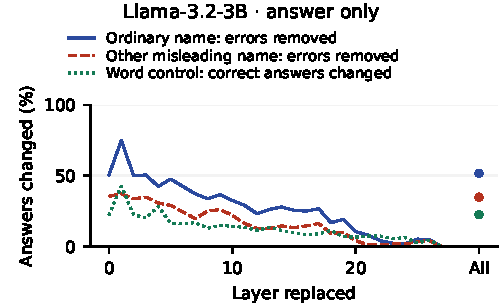
\includegraphics[width=\columnwidth]{figures/a_story_patching.pdf}
\caption{Arithmetic name-site patches, Llama-3.2-3B, queried variable, set 7. All replaces every layer.}
\label{a-fig:patch}
\end{figure}

\begin{figure*}[t]
\centering
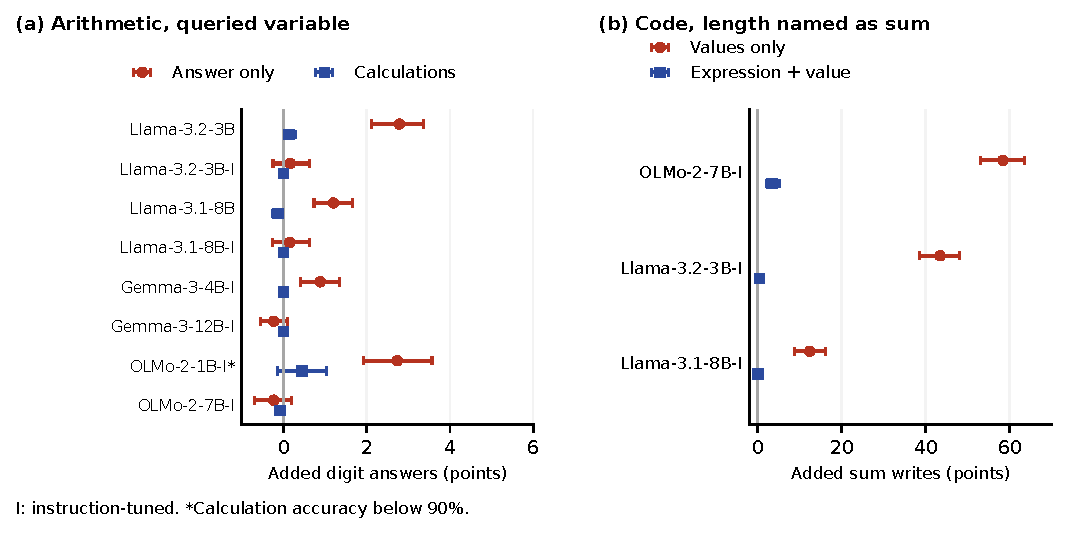
\includegraphics[width=\textwidth]{figures/shared_behavior.pdf}
\caption{Selected name-error contrasts (95\% intervals); scales differ.}
\label{fig:behavior}\label{a-fig:master}
\end{figure*}



\section{Code task levels and identifiers}
\label{c-app:levels}

Levels vary dependency depth, distractors and which assignment receives the misleading name.
The primary comparison uses level~5. A function is generated once; renaming preserves its
statements, input and executable result. Table~\ref{c-tab:gate} lists the operation suggested by
each identifier. Sum and length are admissible name-suggested operations on the aggregate step; minimum
and maximum are excluded because their result is already present in the input.


\begin{table*}[t]
\centering\small
\begin{tabular}{@{}clc@{}}
\toprule
Level & Neutral program (body) & Traced steps \\
\midrule
1 & \texttt{v = len(xs); return v} & 1 \\
2 & \texttt{v = len(xs); w = v * 2; return w} & 2 \\
3 & \texttt{v = len(xs); w = max(xs); u = v + w; return u} & 3 \\
4 & level 3 with an unused fourth assignment & 3 \\
5 & \texttt{v = len(xs); w = v * 2; u = w + 3; return u} & 3 \\
6 & level 5 with the misleading name on the middle step & 3 \\
\bottomrule
\end{tabular}
\caption{The levels, one example each. The aggregate in the first statement is any of
\texttt{len}, \texttt{sum}, \texttt{max}, \texttt{min}; unary operations are \texttt{*2},
\texttt{//2}, \texttt{+c}, \texttt{-c}. The misleading name sits on the first statement at
levels 1--5 and on the second at level 6.}
\label{c-tab:levels}
\end{table*}

\begin{table*}[t]
\centering\small
\begin{tabular}{@{}lll@{}}
\toprule
Family & Names & Implied operation \\
\midrule
len & \texttt{count}, \texttt{n\_items}, \texttt{length} & \texttt{len(xs)} \\
sum & \texttt{total}, \texttt{sum\_all}, \texttt{acc} & \texttt{sum(xs)} \\
max & \texttt{largest}, \texttt{max\_val}, \texttt{peak} & \texttt{max(xs)} \\
min & \texttt{smallest}, \texttt{min\_val}, \texttt{low} & \texttt{min(xs)} \\
double & \texttt{double}, \texttt{twice} & \texttt{2 * a} \\
half & \texttt{half} & \texttt{a // 2} \\
succ & \texttt{succ}, \texttt{next\_val} & \texttt{a + 1} \\
pred & \texttt{pred}, \texttt{prev\_val} & \texttt{a - 1} \\
add & \texttt{combined}, \texttt{both} & \texttt{a + b} \\
sub & \texttt{diff}, \texttt{gap} & \texttt{a - b} \\
mul & \texttt{product}, \texttt{scaled} & \texttt{a * b} \\
\bottomrule
\end{tabular}
\caption{Identifier families and their suggested operations. The gate (Appendix~\ref{c-app:gate}) scores each name by the log-probability each
model assigns to the candidate right-hand sides; \NUM{c-gate-pass} of \NUM{c-gate-names} names are
read as intended by at least 80\% of models. The min and max names cannot produce name errors on the
aggregate step (their value is an input element) and are used as congruent and
alternative-name names.}
\label{c-tab:gate}
\end{table*}

\section{Identifier meanings}
\label{c-app:gate}
For each identifier and model, we compare log-probabilities of candidate right-hand sides after
a prefix such as \texttt{def f(xs):\textbackslash n\ \ \ \ total =}.
The highest-scoring operation records what that identifier evokes. Of \NUM{c-gate-names} names,
\NUM{c-gate-pass} match the intended operation in at least 80\% of models. Most sum-family names
instead evoke length in \NUM{c-gate-sum-len-readers} of \NUM{c-n-models} models. This check matters
when interpreting a small effect: an identifier need not suggest the same operation to every model.
The design planned to retain only names passing the 80\% panel gate. The runs instead retained
the full name table, so the reported comparisons depart from that selection rule. The results
concern these named groups; they do not establish that every model reads each name as intended.

\section{Operation and name pairings}
\label{c-app:matrix}
\begin{table*}[t]
\centering\small
\begin{tabular}{@{}lrrrr@{}}
\toprule
Model & Return acc. & Direct: errors & Trace: len$\to$sum & Trace: max$\to$sum \\
\midrule
OLMo-2-7B & 95.7 & +0.4 & +58.4$^{*}$ [+53.0, +63.5] & +1.9 [+1.1, +3.0] \\
Llama-3.2-3B & 97.4 & +0.8 & +43.4$^{*}$ [+38.5, +48.1] & +0.0 [+0.0, +0.0] \\
Llama-3.1-8B & 99.6 & +0.5 & +12.4$^{*}$ [+8.8, +16.0] & +0.0 [+0.0, +0.0] \\
CodeLlama-7B & 91.7 & +1.0 & +3.7$^{*}$ [+2.2, +5.4] & +10.7$^{*}$ [+7.9, +13.7] \\
CodeGemma-7B & 99.2 & +1.5$^{*}$ & +0.1 [+0.0, +0.4] & +0.0 [+0.0, +0.0] \\
Gemma-3-4B & 99.1 & +0.8 & +0.0 [+0.0, +0.0] & +0.0 [+0.0, +0.0] \\
OLMo-2-1B & 37.8 & +3.1$^{*}$ & +3.7$^{*}$ [+2.2, +5.5] & +4.2$^{*}$ [+2.6, +5.9] \\
CodeLlama-34B & 98.9 & -- & +0.0 [+0.0, +0.0] & +1.8$^{*}$ [+0.7, +3.1] \\
\bottomrule
\end{tabular}

\caption{Full level-5 panel: ordinary-name final-answer accuracy (\%) and excess name errors (points).
Direct contrasts rename the returned variable; trace contrasts rename the first assignment.
Trace columns include 95\% intervals. Stars mark consistent signs and intervals excluding zero.}
\label{c-tab:full-panel}
\end{table*}

Table~\ref{c-tab:matrix} reports all tested aggregate/name pairings. The reverse of the main
length-to-sum conflict is weak at level~5: sum-computed variables with length-like names have
excess within two points for models above the neutral-accuracy floor. At level~3, OLMo-2-7B has
\NUM{c-pair-olmo7-L3-sumlen-excess} points of excess in that pairing.
Gemma-3-4B shows no main-cell effect, consistent with its identifier-meaning check. OLMo-2-1B's
neutral accuracy is only \NUM{c-cell-olmo1-acc}\%, making its small, broadly distributed effects
harder to interpret as a specific trace failure.


\begin{table*}[t]
\centering\small
\begin{tabular}{@{}lrrrrr@{}}
\toprule
Model & len$\to$sum & max$\to$sum & min$\to$sum & sum$\to$len & max$\to$len \\
\midrule
OLMo-2-7B & +17.6$^{*}$ / +58.4$^{*}$ & +0.9 / +1.9 & +0.0 / +0.2 & +4.4$^{*}$ / +0.0 & +0.0 / +0.0 \\
Llama-3.2-3B & +23.6$^{*}$ / +43.4$^{*}$ & +1.1 / +0.0 & +0.0 / +0.0 & +0.0 / +0.0 & +0.0 / +0.0 \\
Llama-3.1-8B & +1.5 / +12.4$^{*}$ & +0.7 / +0.0 & +0.0 / +0.0 & +0.0 / +0.0 & +0.0 / +0.0 \\
CodeLlama-7B & +0.9 / +3.7$^{*}$ & +7.5 / +10.7$^{*}$ & +1.0 / +1.7 & +1.5 / +0.0 & +0.9 / +0.6 \\
CodeGemma-7B & +0.0 / +0.1 & +10.8$^{*}$ / +0.0 & +0.0 / +0.0 & +0.0 / +0.0 & +0.0 / +0.0 \\
Gemma-3-4B & +0.0 / +0.0 & +0.2 / +0.0 & +0.0 / +0.0 & +0.0 / +0.0 & +0.0 / +0.0 \\
OLMo-2-1B & +1.2 / +3.7$^{*}$ & +2.8$^{*}$ / +4.2$^{*}$ & +0.3 / -0.2 & +10.6$^{*}$ / +11.1$^{*}$ & +9.6$^{*}$ / +5.6$^{*}$ \\
\bottomrule
\end{tabular}

\caption{Excess name errors at the aggregate step, trace regime, level 3 / level 5, three
sets of worked examples pooled; $^{*}$ as in Table~\ref{c-tab:full-panel}.}
\label{c-tab:matrix}
\end{table*}

\section{Demonstration formats}
\begin{table*}[t]
\centering\small
\begin{tabular}{@{}llrrr@{}}
\toprule
Example format & Shown value & OLMo-2-7B-I & Llama-3.2-3B-I & Llama-3.1-8B-I \\
\midrule
Values only & \texttt{v = 2} & +58.4 & +43.4 & +12.4 \\
Matched descriptive text & \texttt{v = 2 [notes]} & +56.6 & +49.6 & -- \\
Numeric elaboration & \texttt{v = 2 + 0 = 2} & +41.3 & +14.9 & -- \\
Interactive Python & \texttt{>>> v}\quad\texttt{2} & +9.5 & +12.6 & +0.2 \\
Code comments & \texttt{v = len(xs) \# 2} & +0.0 & +6.8 & +0.1 \\
Expression and value & \texttt{v = len(xs) = 2} & +3.4 & +0.4 & +0.0 \\
\bottomrule
\end{tabular}

\caption{Code format comparison: added sum writes (points). Dashes: untested.}
\label{tab:formats}\label{c-tab:formats}
\end{table*}

\label{c-app:formats}

All few-shot comparisons hold programs, demonstration identities and model weights fixed.
The values-only format writes \texttt{qq = 3}; the expression-and-value format writes
\texttt{qq = len(xs) = 3}; the interactive Python format writes
\texttt{>{}>{}> qq} followed by \texttt{3}; comment mode annotates each assignment with its
value. These are model-generated transcripts, not interpreter executions. Prose asks for step-by-step reasoning without demonstrations. Table~\ref{c-tab:formats-ci}
gives the paired excess and interval for each few-shot format.

On the main conflict, interactive-transcript excess is \NUM{c-cell-olmo7-repl-excess} and
\NUM{c-cell-llama3-repl-excess} points for OLMo-2-7B and Llama-3.2-3B, compared with
\NUM{c-cell-llama8-repl-excess} for Llama-3.1-8B. Comments leave
\NUM{c-cell-llama3-comment-excess} points in Llama-3.2-3B and near-zero excess in the other two.
Prose has little initial name errors, so asking it to state or recompute values does not test
removal of the large trace effect. The prediction that interactive transcripts would stay within a factor of two
of trace was not supported; the comment prediction held only for two models.

The paired trace-minus-trace-expr name-error-rate reductions are \NUM{c-expr-olmo7-drop} points
[\NUM{c-expr-olmo7-drop-lo}, \NUM{c-expr-olmo7-drop-hi}], \NUM{c-expr-llama3-drop}
[\NUM{c-expr-llama3-drop-lo}, \NUM{c-expr-llama3-drop-hi}] and \NUM{c-expr-llama8-drop}
[\NUM{c-expr-llama8-drop-lo}, \NUM{c-expr-llama8-drop-hi}] for OLMo-2-7B, Llama-3.2-3B and
Llama-3.1-8B. These 95\% intervals keep each matched program's demonstration-seed repeats together.


\begin{table*}[t]
\centering\small
\begin{tabular}{@{}llrrr@{}}
\toprule
Format shown in examples & Example & OLMo-2-7B & Llama-3.2-3B & Llama-3.1-8B \\
\midrule
Values only & \texttt{v = 2} & +58.4$^{*}$ [+53.0, +63.5] & +43.4$^{*}$ [+38.5, +48.1] & +12.4$^{*}$ [+8.8, +16.0] \\
Interactive Python transcript & \shortstack[l]{\texttt{>{}>{}> v}\\\texttt{2}} & +9.5$^{*}$ [+6.9, +12.0] & +12.6$^{*}$ [+9.4, +15.9] & +0.2 [+0.0, +0.6] \\
Code with value comments & \texttt{v = len(xs) \# 2} & +0.0 [+0.0, +0.0] & +6.8$^{*}$ [+4.4, +9.2] & +0.1 [+0.0, +0.4] \\
Expression and value & \texttt{v = len(xs) = 2} & +3.4$^{*}$ [+2.0, +5.1] & +0.4 [+0.0, +0.9] & +0.0 [+0.0, +0.0] \\
\bottomrule
\end{tabular}

\caption{Baseline formats with 95\% bootstrap intervals over matched problems.}
\label{c-tab:formats-ci}
\end{table*}

\section{Probe and patching details}
\label{c-app:probes}

\begin{figure*}[t]
\centering
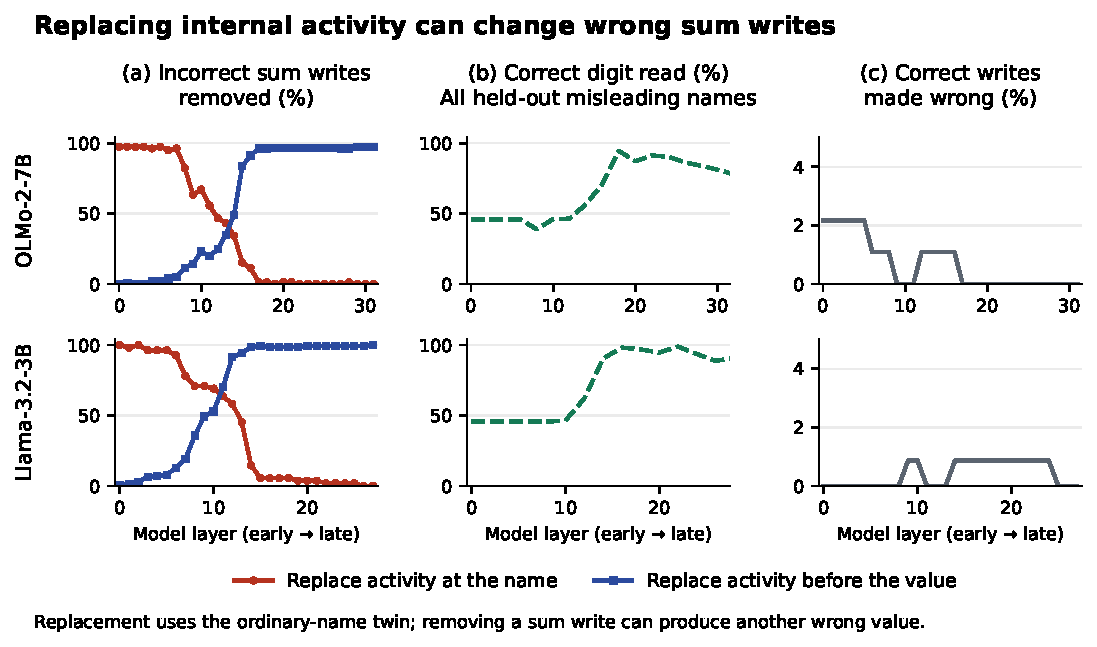
\includegraphics[width=\textwidth]{figures/c_mechanism.pdf}
\caption{\textbf{(a)} Name-error removal. \textbf{(b)} Correct-digit readout.
\textbf{(c)} Damage to correct writes. Patches use ordinary-name twins.}
\label{c-fig:mechanism}
\end{figure*}

We follow \citeauthor{kudo2026faithful}'s 10-class linear-probe recipe, with three seeds and
neutral-only training. Each probe predicts a target digit from one residual-stream position
and layer. Name-identity controls use deterministic random labels keyed on the identifier
\cite{hewitt2019control}. Neutral names and values vary independently, and misleading names
are absent from training. The original implementation reused test programs in training. The reported reruns
replace those scores: they train on \NUM{c-probe-n-train} independent neutral programs and
evaluate \NUM{c-probe-n-test} misleading-name programs, with overlap guards that ignore name
spelling. Table~\ref{c-tab:probe-repeats} reports the name controls alongside digit accuracy.

% Disjoint-probe demonstration repeats
Figure~\ref{c-fig:mechanism}'s probe curves use demonstration set 7. Repeating training and evaluation with sets 11 and 13
gives true-digit accuracies of \NUM{c-probe-olmo7-demo-lo}--\NUM{c-probe-olmo7-demo-hi}\%,
\NUM{c-probe-llama3-demo-lo}--\NUM{c-probe-llama3-demo-hi}\% and
\NUM{c-probe-llama8-demo-lo}--\NUM{c-probe-llama8-demo-hi}\% across the three sets. Each repeat
uses the same independent training programs and three probe seeds; its layer is selected by
that set's neutral accuracy. These repeats assess prompt sensitivity, not a causal role for
the decoded digit. Table~\ref{c-tab:probe-repeats} gives both conditions' readouts and controls.

\begin{table*}[t]
\centering\small
\begin{tabular}{@{}lrrrrrrr@{}}
\toprule
Model & Set & Layer & Neutral & Control & Misleading & Control & Majority \\
\midrule
OLMo-2-7B & 7 & 18 & 99.5 & 100.0 & 94.5 & 33.0 & 45.6 \\
OLMo-2-7B & 11 & 18 & 97.3 & 100.0 & 95.4 & 0.0 & 45.6 \\
OLMo-2-7B & 13 & 18 & 99.8 & 100.0 & 97.4 & 23.4 & 45.6 \\
Llama-3.2-3B & 7 & 24 & 98.8 & 99.7 & 93.7 & 20.0 & 45.6 \\
Llama-3.2-3B & 11 & 20 & 100.0 & 99.8 & 95.4 & 5.0 & 45.6 \\
Llama-3.2-3B & 13 & 28 & 99.4 & 100.0 & 99.9 & 1.9 & 45.6 \\
Llama-3.1-8B & 7 & 16 & 100.0 & 87.8 & 99.9 & 33.0 & 45.6 \\
Llama-3.1-8B & 11 & 20 & 100.0 & 81.6 & 100.0 & 0.1 & 45.6 \\
Llama-3.1-8B & 13 & 20 & 100.0 & 87.2 & 100.0 & 3.0 & 45.6 \\
\bottomrule
\end{tabular}

\caption{Disjoint code probes, three demonstration sets. Neutral and misleading are
true-digit accuracy; each control column gives name-identity accuracy for that condition.
Majority predicts the most frequent digit in training on the misleading test programs.
Rates are percentages, averaged over three probe seeds. Layers are selected by neutral accuracy.}
\label{c-tab:probe-repeats}
\end{table*}

We supply the correct trace token by token when caching probe inputs. The decision position is the \texttt{=} before the
first traced value; later values cannot affect this position under causal attention. Patching
uses only the prompt and this trace prefix. Name patches replace every aligned
occurrence of the identifier; decision patches replace only that writing position. Both use
one layer at a time and include a neutral-for-neutral disruption control
\cite{zhang2024patching}. The alternative-name control is uninformative in the main cell:
every sum-family identifier implies the same sum, so there is no distinct source name-suggested value.
Llama-3.1-8B's affected two-token name lacks aligned neutral twins for the name-site intervention.


\begin{table*}[t]
\centering\small
\begin{tabular}{@{}lrrrrrrr@{}}
\toprule
& \multicolumn{3}{c}{Name tokens} & \multicolumn{4}{c}{Decision token} \\ \cmidrule(lr){2-4}\cmidrule(lr){5-8}
Model & L0 & damage & $<$10\% by & 50\% at & 90\% at & all layers & damage \\
\midrule
OLMo-2-7B & 97\% & 2\% & L17 & L15 & L16 & 97\% & 2\% \\
Llama-3.2-3B & 100\% & 0\% & L15 & L10 & L12 & 100\% & 0\% \\
Llama-3.1-8B & -- & -- & -- & L8 & L9 & 100\% & 0\% \\
\bottomrule
\end{tabular}

\caption{Layers behind Figure~\ref{c-fig:mechanism}. Name tokens: name errors removed by
replacing every token of the name at layer 0, damage to correct instances, and the first
layer after which removal falls below 10\%. Decision token: first layer at which a
single-layer replacement removes 50\% and 90\% of name errors, removal with every layer
replaced, and its damage. Llama-3.1-8B's name errors fall on a two-token name without a
token-aligned twin.}
\label{c-tab:patch}
\end{table*}

\section{Scope checks}
\label{c-app:boundaries}

\paragraph{Operation and scale.} Moving the misleading name to a unary middle step produces
no reliable effect for models above the accuracy floor; the largest excess is
\NUM{c-l6-max-excess} points. CodeLlama-34B's length-to-sum effect is \NUM{c-cell34-len-excess},
while its maximum-to-sum effect is \NUM{c-cell34-max-excess} points
[\NUM{c-cell34-max-lo}, \NUM{c-cell34-max-hi}]. The latter is a reliable positive effect, but its
interval extends beyond the two-point margin. Its small point estimate cannot be reported as
equivalence. The larger-checkpoint result supports the registered maximum-to-sum direction
and reliable-effect criterion, while its magnitude is much smaller than CodeLlama-7B's.

\paragraph{Natural code.} We select \NUM{c-crux-n} CRUXEval functions with length, loop-counter
or maximum assignments, rename the target by AST rewriting to \texttt{v} or \texttt{total},
and verify execution after renaming. Direct and prose accuracy contrasts all have intervals
covering zero on the \NUM{c-crux-used} functions whose renamed target is used downstream.
Their endpoints stay within \NUM{c-crux-direct-bound} and
\NUM{c-crux-prose-bound} points, respectively (Table~\ref{c-tab:crux}). These are bounded results
for those functions and prompts; they do not test the trace that lists values without expressions used in the synthetic
study.
The natural-code functions come from \citet{gu2024cruxeval}.


\begin{table*}[t]
\centering\small
\begin{tabular}{@{}lrrrr@{}}
\toprule
Model & Direct acc. & Direct $\Delta$ & Prose acc. & Prose $\Delta$ \\
\midrule
OLMo-2-7B & 10 & +1.2 [+0.0, +3.6] & 22 & -1.2 [-9.5, +8.3] \\
Llama-3.2-3B & 19 & +1.2 [-2.4, +4.8] & 25 & +3.6 [-3.6, +10.7] \\
Llama-3.1-8B & 22 & -3.6 [-9.5, +2.4] & 40 & +0.0 [-9.5, +9.5] \\
CodeLlama-7B & 18 & +2.4 [+0.0, +6.0] & 13 & +2.4 [-4.8, +9.5] \\
CodeGemma-7B & 18 & +0.0 [-4.8, +4.8] & 22 & +2.4 [-8.3, +13.1] \\
Gemma-3-4B & 15 & -2.4 [-6.0, +0.0] & 45 & +4.8 [-1.2, +11.9] \\
OLMo-2-1B & 16 & -3.6 [-8.3, +0.0] & 3 & +6.0 [+0.0, +11.9] \\
\bottomrule
\end{tabular}

\caption{\NUM{c-crux-n} CRUXEval functions that assign a variable from \texttt{len(\ldots)}
(\NUM{c-crux-kind-len}), a loop counter (\NUM{c-crux-kind-counter}) or \texttt{max(\ldots)}
(\NUM{c-crux-kind-max}), of which \NUM{c-crux-used} use it downstream; each rendered with the
original name, the neutral name \texttt{v}, and the misleading name \texttt{total}. Accuracy
on all neutral renderings, and the paired misleading-minus-neutral difference in points on
the downstream-used subset, with a bootstrap interval over functions.}
\label{c-tab:crux}
\end{table*}


\section{Effect and equivalence checks}
\label{c-app:stats}
Each contrast subtracts the neutral twin's rate for the same digit. We resample matched problems
with demonstration-seed replicates together and use 95\% cluster-bootstrap intervals.
Reliability also requires a consistent sign across all three demonstration sets.

Equivalence applies the $\pm\NUM{c-eq-delta}$-point margin to 90\% intervals from the same
cluster bootstrap (two one-sided 5\% tests), using 2,000 draws. Across \NUM{c-eq-cells} tested contrasts,
\NUM{c-eq-equivalent} intervals lie wholly inside the margin, \NUM{c-eq-witheffect} contrasts have
reliable effects without meeting that bound, and \NUM{c-eq-inconclusive} meet neither criterion.
A small estimate or an interval covering zero does not by itself establish equivalence.

% Generated by scripts/77_followup_tables.py from validated JSON.
\section{Generated-prefix audit and initial readouts}
\label{c-app:round5-errors}
For 2565 of 2565 misleading-name generations, the token prefix through the marker before the first value exactly matches the cached trace. This verifies that the cached state at that marker also precedes the generated value. No target value token is included.
These initial readouts select layers on the full neutral evaluation set; the main text instead uses independent cross-fitted selection (Appendix~\ref{c-app:round6-probes}). We split the generated writes into name-suggested values, correct values and other errors. Table~\ref{c-tab:round5-errors} averages three probe seeds and pools demonstration sets 7, 11 and 13. Intervals resample matched programs with all their demonstration repeats (4,000 draws). These conditional readouts establish available information on observed errors; they do not establish its causal use.
\begin{table*}[t]
\centering\small
\sbox{\roundfivebox}{\begin{tabular}{@{}llrrl@{}}
\toprule
Model & Generated write & Rows & Programs & True-digit accuracy (\%) \\
\midrule
OLMo-2-7B & name error & 503 & 193 & 96.4 [94.8, 97.8] \\
OLMo-2-7B & correct write & 320 & 135 & 96.7 [94.4, 98.5] \\
OLMo-2-7B & other error & 32 & 24 & 77.1 [61.7, 90.5] \\
Llama-3.2-3B & name error & 372 & 169 & 95.7 [93.8, 97.4] \\
Llama-3.2-3B & correct write & 440 & 204 & 98.3 [97.0, 99.3] \\
Llama-3.2-3B & other error & 43 & 29 & 82.2 [71.2, 91.7] \\
Llama-3.1-8B & name error & 106 & 45 & 99.7 [99.0, 100.0] \\
Llama-3.1-8B & correct write & 749 & 261 & 100.0 [100.0, 100.0] \\
Llama-3.1-8B & other error & 0 & 0 & -- \\
\bottomrule
\end{tabular}}
\ifdim\wd\roundfivebox>\textwidth\resizebox{\textwidth}{!}{\usebox{\roundfivebox}}\else\usebox{\roundfivebox}\fi
\caption{Disjoint probes at the verified generated prefix. A dash denotes an empty stratum. The denominator is observed writes within each stratum, not independent demonstration repeats.}
\label{c-tab:round5-errors}
\end{table*}
\section{Sensitivity to identifier meanings}
\label{c-app:round5-identifiers}
None of the three main-cell names (\texttt{total}, \texttt{sum\_all}, \texttt{acc}) meets the originally planned 80\% panel gate. Its filtered estimate is therefore unavailable, rather than zero.
Table~\ref{c-tab:round5-identifiers} retains the full-data estimate and reports each name and each model's own meaning gate. Gates use the original saved meaning checks. Intervals cluster matched programs across the three demonstration sets. This exploratory sensitivity does not replace the planned panel gate or remove the deviation from it.
\begin{table*}[t]
\centering\small
\sbox{\roundfivebox}{\begin{tabular}{@{}llllll@{}}
\toprule
Model & All & Model gate & \texttt{total} & \texttt{sum\_all} & \texttt{acc} \\
\midrule
Gemma-3-4B & 0.0 [0.0, 0.0] & -- & 0.0 [0.0, 0.0] & 0.0 [0.0, 0.0] & 0.0 [0.0, 0.0] \\
CodeGemma-7B & 0.1 [0.0, 0.4] & 0.1 [0.0, 0.4] & 0.0 [0.0, 0.0] & 0.3 [0.0, 1.0] & 0.0 [0.0, 0.0] \\
Llama-3.1-8B & 12.4 [8.9, 16.0] & 12.4 [8.9, 16.0] & 0.0 [0.0, 0.0] & 34.0 [26.0, 42.3] & 0.0 [0.0, 0.0] \\
OLMo-2-1B & 3.7 [2.2, 5.5] & 5.0 [1.8, 8.9] & 5.0 [1.8, 8.9] & 5.8 [2.6, 9.3] & 0.0 [0.0, 0.0] \\
OLMo-2-7B & 58.4 [53.1, 63.4] & 59.3 [52.7, 65.8] & 56.4 [47.9, 64.9] & 96.2 [93.9, 98.1] & 15.3 [9.6, 21.8] \\
CodeLlama-7B & 3.7 [2.1, 5.5] & 3.7 [2.1, 5.5] & 1.8 [0.4, 3.2] & 8.7 [4.5, 13.1] & 0.0 [0.0, 0.0] \\
Llama-3.2-3B & 43.4 [38.5, 48.0] & 43.4 [38.5, 48.0] & 30.1 [23.8, 36.9] & 76.3 [70.2, 82.4] & 18.4 [11.9, 25.7] \\
\bottomrule
\end{tabular}}
\ifdim\wd\roundfivebox>\textwidth\resizebox{\textwidth}{!}{\usebox{\roundfivebox}}\else\usebox{\roundfivebox}\fi
\caption{Excess name errors in percentage points [95\% interval], level 5 length-to-sum. Empty subsets are shown as dashes. The saved JSON also reports each demonstration set and the all-three-sets sign rule.}
\label{c-tab:round5-identifiers}
\end{table*}
\section{Length and numeric elaboration controls}
\label{c-app:round5-formats}
We add neutral annotations to each demonstrated value, matching the expression demonstrations' token counts, and separately add valid numeric elaborations of the form \texttt{name = value + 0 = value}. The test program and \texttt{Trace:} prefix are unchanged. Greedy decoding uses the same 285 misleading programs and neutral twins for each format. Table~\ref{c-tab:round5-formats} pools three demonstration sets; changes relative to the original trace and expression trace are paired on the same programs.
The length-matched annotation controls retain much larger excess than expression demonstrations in both models. Numeric elaboration reduces excess relative to the original trace but leaves a larger effect than source expressions. Token count alone does not reproduce the expression benefit, and adding valid arithmetic accounts for part of it; these two contrasts do not isolate a single mechanism.
\begin{table*}[t]
\centering\small
\sbox{\roundfivebox}{\begin{tabular}{@{}lllll@{}}
\toprule
Model & Format & Excess & Change vs trace & Change vs expression \\
\midrule
OLMo-2-7B & neutral annotation & 56.6 [51.3, 61.6] & -1.8 [-3.4, -0.1] & 53.2 [48.1, 58.2] \\
OLMo-2-7B & numeric elaboration & 41.3 [36.4, 46.0] & -17.1 [-21.1, -12.9] & 37.9 [33.2, 42.5] \\
Llama-3.2-3B & neutral annotation & 49.6 [44.7, 54.3] & 6.2 [4.1, 8.4] & 49.2 [44.3, 53.9] \\
Llama-3.2-3B & numeric elaboration & 14.9 [12.0, 17.8] & -28.5 [-32.7, -24.3] & 14.5 [11.7, 17.4] \\
\bottomrule
\end{tabular}}
\ifdim\wd\roundfivebox>\textwidth\resizebox{\textwidth}{!}{\usebox{\roundfivebox}}\else\usebox{\roundfivebox}\fi
\caption{Excess name errors and paired changes in percentage points [95\% interval]. Bootstrap clusters keep all demonstration repeats for each matched program together. These controls assess length and numeric elaboration; they do not by themselves establish how expressions change generation.}
\label{c-tab:round5-formats}
\end{table*}

% Generated from validated round-six summaries.
\section{Independent probe layer selection}
\label{c-app:round6-probes}
The main-text error readouts use five-fold cross-fitting. A fixed SHA256 hash assigns canonical program computations to folds, keeping renamed versions and demonstration repeats together. For each held-out fold, we select the layer with the highest neutral accuracy on the other four folds, averaging three probe seeds and breaking ties toward the lowest layer. Neither the held-out neutral labels nor its misleading writes enter that choice. Probe training remains disjoint from every evaluation computation.
Each program is scored only with its held-out fold's layer. The generated-prefix audit from Appendix~\ref{c-app:round5-errors} still applies. Table~\ref{c-tab:round6-probes} reports the conditional write strata and paired changes from the earlier full-neutral selection. Intervals use 4,000 canonical-program bootstrap draws, keeping demonstration repeats together. They condition on the fixed fold selectors and do not refit layer selection inside each bootstrap. Name controls and the full layer curves remain descriptive measurements in Appendix~\ref{c-app:probes}.
\begin{table*}[t]
\centering\small
\sbox{\roundsixbox}{\begin{tabular}{@{}llrrll@{}}
\toprule
Model & Write & Rows & Computations & Accuracy (\%) & Change (points) \\
\midrule
OLMo-2-7B & name error & 503 & 193 & 96.4 [94.9, 97.9] & 0.0 [0.0, 0.0] \\
OLMo-2-7B & correct write & 320 & 135 & 96.7 [94.4, 98.4] & 0.0 [0.0, 0.0] \\
OLMo-2-7B & other error & 32 & 24 & 77.1 [61.6, 90.6] & 0.0 [0.0, 0.0] \\
Llama-3.2-3B & name error & 372 & 169 & 95.5 [93.6, 97.3] & -0.2 [-0.9, 0.4] \\
Llama-3.2-3B & correct write & 440 & 204 & 98.0 [96.6, 99.1] & -0.3 [-0.8, 0.0] \\
Llama-3.2-3B & other error & 43 & 29 & 82.2 [71.1, 91.7] & 0.0 [0.0, 0.0] \\
Llama-3.1-8B & name error & 106 & 45 & 99.7 [99.0, 100.0] & 0.0 [0.0, 0.0] \\
Llama-3.1-8B & correct write & 749 & 261 & 100.0 [99.9, 100.0] & -0.0 [-0.1, 0.0] \\
Llama-3.1-8B & other error & 0 & 0 & -- & -- \\
\bottomrule
\end{tabular}}
\ifdim\wd\roundsixbox>\textwidth\resizebox{\textwidth}{!}{\usebox{\roundsixbox}}\else\usebox{\roundsixbox}\fi
\caption{True-digit readouts with independent layer selection. Changes compare the same observed writes with the earlier full-neutral layer choice. A dash denotes an empty stratum. These readouts establish decodability, not causal use.}
\label{c-tab:round6-probes}
\end{table*}
\section{Independent replication with screened names}
\label{c-app:round6-identifiers}
We fix \NUM{c-r6-screen-n} fresh sum-family candidates before scoring them with the original candidate-continuation meaning check (Appendix~\ref{c-app:gate}). The panel is the same seven models used for that gate. A name qualifies when sum is the highest-scoring continuation in at least 80\% of the panel; ties follow the original scoring order. Two additional function-name contexts and neutral names are diagnostic and do not affect selection. Of the candidates, \NUM{c-r6-screen-passed} qualify. We freeze the first \NUM{c-r6-name-n} qualifying names in the fixed order: \NUM{c-r6-name-list}. No trace outcomes enter selection.
The replication uses \NUM{c-r6-program-n} new length-computed programs. Their canonical computations are unique and absent from the original level-5 training and test corpus and all three demonstration sets. True and name-suggested values are checked by execution and retain the original value-exclusion rules. Every selected name is crossed with every program; its neutral twin differs only in the target identifier. The three affected models and the prespecified CodeGemma-7B control use the same programs and demonstration sets 7, 11 and 13 under trace and expression demonstrations.
Table~\ref{c-tab:round6-replication} pools names and demonstration sets, clustering all repeats of each computation in 4,000 bootstrap draws. Table~\ref{c-tab:round6-replication-names} reports each identifier. The format contrast replicates on independently selected names, but names and programs differ from the original experiment, so differences in effect magnitude across the two samples are descriptive. This exploratory replication does not retroactively repair the original selection-rule deviation. Probes and patches concern the original identifiers, not these new names.
\begin{table*}[t]
\centering\small
\sbox{\roundsixbox}{\begin{tabular}{@{}lccc@{}}
\toprule
Candidate & Sum agreement & Qualifies & Selected \\
\midrule
\texttt{sum\_of\_values} & 6/7 & yes & yes \\
\texttt{sum\_of\_items} & 7/7 & yes & yes \\
\texttt{sum\_of\_elements} & 7/7 & yes & yes \\
\texttt{sum\_of\_xs} & 7/7 & yes & no \\
\texttt{sum\_of\_list} & 6/7 & yes & no \\
\texttt{list\_sum} & 6/7 & yes & no \\
\texttt{input\_sum} & 6/7 & yes & no \\
\texttt{items\_sum} & 6/7 & yes & no \\
\texttt{elements\_sum} & 5/7 & no & no \\
\texttt{sum\_values} & 5/7 & no & no \\
\texttt{sum\_result} & 6/7 & yes & no \\
\texttt{sum\_total} & 6/7 & yes & no \\
\texttt{total\_sum} & 6/7 & yes & no \\
\texttt{xs\_sum} & 7/7 & yes & no \\
\texttt{sum\_xs} & 7/7 & yes & no \\
\texttt{summation} & 6/7 & yes & no \\
\bottomrule
\end{tabular}}
\ifdim\wd\roundsixbox>\textwidth\resizebox{\textwidth}{!}{\usebox{\roundsixbox}}\else\usebox{\roundsixbox}\fi
\caption{The entire fixed candidate list, in selection order. Qualification uses the original canonical meaning prompt. Selection retains the first three qualifying candidates without consulting behavior.}
\label{c-tab:round6-screen}
\end{table*}
\begin{table*}[t]
\centering\small
\sbox{\roundsixbox}{\begin{tabular}{@{}llll@{}}
\toprule
Model & Trace excess & Expression excess & Expression minus trace \\
\midrule
OLMo-2-7B & 91.1 [88.4, 93.6] & 0.8 [0.3, 1.3] & -90.3 [-92.9, -87.6] \\
Llama-3.2-3B & 61.5 [56.1, 66.9] & 0.0 [0.0, 0.0] & -61.5 [-66.9, -56.1] \\
Llama-3.1-8B & 16.7 [12.8, 20.8] & 0.0 [0.0, 0.0] & -16.7 [-20.8, -12.8] \\
CodeGemma-7B & 0.0 [0.0, 0.0] & 0.0 [0.0, 0.0] & 0.0 [0.0, 0.0] \\
\bottomrule
\end{tabular}}
\ifdim\wd\roundsixbox>\textwidth\resizebox{\textwidth}{!}{\usebox{\roundsixbox}}\else\usebox{\roundsixbox}\fi
\caption{Independent screened-name replication: excess name errors and paired format changes in percentage points [95\% interval]. All selected identifiers and three demonstration sets are pooled over 200 fresh computations. A zero bootstrap interval records no observed paired name errors; it is not a population-level absence or equivalence claim.}
\label{c-tab:round6-replication}
\end{table*}
\begin{table*}[t]
\centering\small
\sbox{\roundsixbox}{\begin{tabular}{@{}llll@{}}
\toprule
Model & Identifier & Trace excess & Expression excess \\
\midrule
OLMo-2-7B & \texttt{sum\_of\_values} & 91.7 [88.8, 94.3] & 0.2 [0.0, 0.5] \\
OLMo-2-7B & \texttt{sum\_of\_items} & 89.2 [86.0, 92.0] & 2.0 [0.8, 3.3] \\
OLMo-2-7B & \texttt{sum\_of\_elements} & 92.5 [89.8, 94.8] & 0.2 [0.0, 0.5] \\
Llama-3.2-3B & \texttt{sum\_of\_values} & 61.7 [56.0, 67.3] & 0.0 [0.0, 0.0] \\
Llama-3.2-3B & \texttt{sum\_of\_items} & 55.5 [50.0, 61.3] & 0.0 [0.0, 0.0] \\
Llama-3.2-3B & \texttt{sum\_of\_elements} & 67.3 [61.7, 73.0] & 0.0 [0.0, 0.0] \\
Llama-3.1-8B & \texttt{sum\_of\_values} & 12.8 [9.3, 16.7] & 0.0 [0.0, 0.0] \\
Llama-3.1-8B & \texttt{sum\_of\_items} & 22.8 [18.0, 27.7] & 0.0 [0.0, 0.0] \\
Llama-3.1-8B & \texttt{sum\_of\_elements} & 14.5 [10.5, 18.7] & 0.0 [0.0, 0.0] \\
CodeGemma-7B & \texttt{sum\_of\_values} & 0.0 [0.0, 0.0] & 0.0 [0.0, 0.0] \\
CodeGemma-7B & \texttt{sum\_of\_items} & 0.0 [0.0, 0.0] & 0.0 [0.0, 0.0] \\
CodeGemma-7B & \texttt{sum\_of\_elements} & 0.0 [0.0, 0.0] & 0.0 [0.0, 0.0] \\
\bottomrule
\end{tabular}}
\ifdim\wd\roundsixbox>\textwidth\resizebox{\textwidth}{!}{\usebox{\roundsixbox}}\else\usebox{\roundsixbox}\fi
\caption{Per-identifier replication, pooling the same three demonstration sets. Effects are percentage points [95\% canonical-program bootstrap interval]. All affected-model trace means are positive in every demonstration set; per-set estimates are retained in the saved summary.}
\label{c-tab:round6-replication-names}
\end{table*}

\section{Prompt-end versus pre-write readouts}
\label{c-app:prompt-comparison}
We fit separate probes at the final token of the complete prompt ending in \texttt{Trace:}, before generating any trace token. Tokenization of this prefix is checked against the original continuation. Training computations, demonstration sets, SGD recipe and seeds match the pre-write probes. Each position selects its layer independently using the same five canonical-computation folds and other folds' neutral labels. Outcome strata and generated-prefix eligibility are frozen from the previous audit. Intervals use 4,000 paired canonical-computation bootstrap draws and condition on the fixed selectors.
\begin{table*}[t]
\centering\small
\sbox{\centralbox}{\begin{tabular}{@{}llrrrrr@{}}
\toprule
Model & Write & Rows / computations & Prompt & Before write & Change & Name ID \\
\midrule
OLMo-2-7B & sum write & 503 / 193 & 38.4 [32.9, 43.9] & 96.4 [94.9, 97.9] & +58.1 [+52.6, +63.4] & 12.7 [9.8, 15.9] \\
OLMo-2-7B & correct write & 320 / 135 & 35.2 [27.7, 43.1] & 96.7 [94.4, 98.4] & +61.5 [+53.3, +69.3] & 20.8 [15.5, 26.3] \\
OLMo-2-7B & other error & 32 / 24 & 76.0 [58.1, 90.2] & 77.1 [61.6, 90.6] & +1.0 [-19.6, +22.6] & 26.0 [12.6, 41.1] \\
Llama-3.2-3B & sum write & 372 / 169 & 26.4 [22.4, 30.8] & 95.5 [93.6, 97.3] & +69.1 [+64.5, +73.4] & 0.7 [0.1, 1.6] \\
Llama-3.2-3B & correct write & 440 / 204 & 37.9 [32.1, 43.7] & 98.0 [96.6, 99.1] & +60.1 [+54.4, +65.8] & 3.6 [1.8, 5.7] \\
Llama-3.2-3B & other error & 43 / 29 & 20.9 [11.7, 31.7] & 82.2 [71.1, 91.7] & +61.2 [+46.8, +73.8] & 2.3 [0.0, 6.1] \\
Llama-3.1-8B & sum write & 106 / 45 & 56.0 [47.4, 64.2] & 99.7 [99.0, 100.0] & +43.7 [+35.4, +52.4] & 0.0 [0.0, 0.0] \\
Llama-3.1-8B & correct write & 749 / 261 & 49.9 [45.7, 54.1] & 100.0 [99.9, 100.0] & +50.1 [+45.8, +54.3] & 0.0 [0.0, 0.0] \\
Llama-3.1-8B & other error & 0 / 0 & -- & -- & -- & -- \\
\bottomrule
\end{tabular}}
\ifdim\wd\centralbox>\textwidth\resizebox{\textwidth}{!}{\usebox{\centralbox}}\else\usebox{\centralbox}\fi
\caption{Paired true-digit accuracies and prompt-position name-identity controls (\%) [95\% interval]. Change is pre-write minus prompt accuracy in points.}
\label{c-tab:prompt-comparison}
\end{table*}

\section{Reproducibility and model terms}
\label{c-app:reproducibility}

The main panel contains seven instruction-tuned checkpoints, with CodeLlama-34B as a
scale check. We use CodeLlama \citep{roziere2023codellama}, CodeGemma
\citep{codegemmateam2024codegemma}, Llama~3 \citep{grattafiori2024llama3}, Gemma~3
\citep{gemmateam2025gemma3} and OLMo~2 \citep{olmo2024olmo2,walsh2025olmo2}.
The model identifiers are \texttt{codellama/CodeLlama-7b-Instruct-hf} and its 34b variant,
\texttt{google/codegemma-7b-it}, \texttt{meta-llama/Llama-3.2-3B-Instruct},
\texttt{meta-llama/Llama-3.1-8B-Instruct}, \texttt{google/gemma-3-4b-it},
\texttt{allenai/OLMo-2-0425-1B-Instruct} and \texttt{allenai/OLMo-2-1124-7B-Instruct}.
These use the Llama~2/CodeLlama, Llama~3.1 or 3.2 Community Licenses, Gemma Terms of Use,
and Apache~2.0, respectively. The study uses their released weights for research inference
and does not redistribute weights. CRUXEval uses the MIT license.

Synthetic data consist of digits, generated identifiers and short Python functions,
without personal records or human annotations. Each tested level has 1,000 matched
problems per target. Main behavior uses three sets of three demonstrations with seeds
7, 11 and 13; programs and demonstration identities remain fixed across compared formats.
Greedy decoding uses the full vocabulary. Parsers retain failed outputs in denominators;
trace-error measurements use the first assignment, while final-answer accuracy scores
the reported return value. Probe training and testing are disjoint in arithmetic computation,
ignoring identifier spelling. The independent-name replication uses separate screened
names and 200 new computations, as described in Appendix~\ref{c-app:round6-identifiers}.

Probes use full-batch SGD with learning rate $10^{-3}$ for 10,000 epochs and seeds 0, 1 and 2.
Five-fold layer selection is disjoint in computation; bootstrap intervals condition on
those selectors. These are linear-predictor fits, not language-model training.
Combined recorded allocations across the arithmetic and code experiments total
\NUM{c-compute-shared-gpuh} GPU-hours on NVIDIA A30, H100 and H200 GPUs, an upper bound
including idle and shared workers. Software is PyTorch~2.11.0 (CUDA~12.9)
\citep{paszke2019pytorch}, Transformers~5.14.1 \citep{wolf2020transformers},
NumPy~2.3.5 and scikit-learn~1.9.1 \citep{pedregosa2011sklearn}.



\begin{table*}[t]
\centering\small
% Generated by scripts/83_main_evidence.py from validated summaries.
\sbox{\centralbox}{\begin{tabular}{@{}lrrrr@{}}
\toprule
Model & \shortstack{Extra sum writes\\(points)} & \shortstack{Correct digit (\%)\\Before trace} & \shortstack{Correct digit (\%)\\Before wrong value} & \shortstack{Wrong writes\\(unique programs)} \\
\midrule
OLMo-2-7B & +58.4 & 38.4 [32.9, 43.9] & 96.4 [94.9, 97.9] & 503 (193) \\
Llama-3.2-3B & +43.4 & 26.4 [22.4, 30.8] & 95.5 [93.6, 97.3] & 372 (169) \\
Llama-3.1-8B & +12.4 & 56.0 [47.4, 64.2] & 99.7 [99.0, 100.0] & 106 (45) \\
\bottomrule
\end{tabular}}
\ifdim\wd\centralbox>\textwidth\resizebox{\textwidth}{!}{\usebox{\centralbox}}\else\usebox{\centralbox}\fi

\caption{Code behavior and error-conditioned readouts [95\% interval]. Counts distinguish writes from computations.}
\label{c-tab:central}
\end{table*}

\section{Correctness on the matched code format cohort}
\label{app:format-correctness}
We score the first written value and final answer on the same 285 original length-to-sum programs and their ordinary-name twins, under values-only and expression-and-value examples. Each format has 855 paired observations over three demonstration sets. Parse failures count as incorrect. Intervals use 4,000 bootstrap draws over matched program IDs, keeping all demonstration repeats and both names together. The format changes are paired on those same IDs. These are overall correctness rates within the specified cohort, rather than the larger task pool. Zero-width intervals record this sample, not certainty about population rates.
\begin{table*}[t]\centering\small
\begin{tabular}{@{}lllrr@{}}
\toprule
Model & Examples & Names & Correct first value (\%) & Correct final answer (\%) \\
\midrule
OLMo-2-7B-I & Values only & Ordinary & \NUM{j-format-olmo7-values-ordinary-first-mean} [\NUM{j-format-olmo7-values-ordinary-first-lo}, \NUM{j-format-olmo7-values-ordinary-first-hi}] & \NUM{j-format-olmo7-values-ordinary-final-mean} [\NUM{j-format-olmo7-values-ordinary-final-lo}, \NUM{j-format-olmo7-values-ordinary-final-hi}] \\
OLMo-2-7B-I & Values only & Misleading & \NUM{j-format-olmo7-values-misleading-first-mean} [\NUM{j-format-olmo7-values-misleading-first-lo}, \NUM{j-format-olmo7-values-misleading-first-hi}] & \NUM{j-format-olmo7-values-misleading-final-mean} [\NUM{j-format-olmo7-values-misleading-final-lo}, \NUM{j-format-olmo7-values-misleading-final-hi}] \\
OLMo-2-7B-I & Expression + value & Ordinary & \NUM{j-format-olmo7-expression-ordinary-first-mean} [\NUM{j-format-olmo7-expression-ordinary-first-lo}, \NUM{j-format-olmo7-expression-ordinary-first-hi}] & \NUM{j-format-olmo7-expression-ordinary-final-mean} [\NUM{j-format-olmo7-expression-ordinary-final-lo}, \NUM{j-format-olmo7-expression-ordinary-final-hi}] \\
OLMo-2-7B-I & Expression + value & Misleading & \NUM{j-format-olmo7-expression-misleading-first-mean} [\NUM{j-format-olmo7-expression-misleading-first-lo}, \NUM{j-format-olmo7-expression-misleading-first-hi}] & \NUM{j-format-olmo7-expression-misleading-final-mean} [\NUM{j-format-olmo7-expression-misleading-final-lo}, \NUM{j-format-olmo7-expression-misleading-final-hi}] \\
\addlinespace
Llama-3.2-3B-I & Values only & Ordinary & \NUM{j-format-llama3-values-ordinary-first-mean} [\NUM{j-format-llama3-values-ordinary-first-lo}, \NUM{j-format-llama3-values-ordinary-first-hi}] & \NUM{j-format-llama3-values-ordinary-final-mean} [\NUM{j-format-llama3-values-ordinary-final-lo}, \NUM{j-format-llama3-values-ordinary-final-hi}] \\
Llama-3.2-3B-I & Values only & Misleading & \NUM{j-format-llama3-values-misleading-first-mean} [\NUM{j-format-llama3-values-misleading-first-lo}, \NUM{j-format-llama3-values-misleading-first-hi}] & \NUM{j-format-llama3-values-misleading-final-mean} [\NUM{j-format-llama3-values-misleading-final-lo}, \NUM{j-format-llama3-values-misleading-final-hi}] \\
Llama-3.2-3B-I & Expression + value & Ordinary & \NUM{j-format-llama3-expression-ordinary-first-mean} [\NUM{j-format-llama3-expression-ordinary-first-lo}, \NUM{j-format-llama3-expression-ordinary-first-hi}] & \NUM{j-format-llama3-expression-ordinary-final-mean} [\NUM{j-format-llama3-expression-ordinary-final-lo}, \NUM{j-format-llama3-expression-ordinary-final-hi}] \\
Llama-3.2-3B-I & Expression + value & Misleading & \NUM{j-format-llama3-expression-misleading-first-mean} [\NUM{j-format-llama3-expression-misleading-first-lo}, \NUM{j-format-llama3-expression-misleading-first-hi}] & \NUM{j-format-llama3-expression-misleading-final-mean} [\NUM{j-format-llama3-expression-misleading-final-lo}, \NUM{j-format-llama3-expression-misleading-final-hi}] \\
\addlinespace
Llama-3.1-8B-I & Values only & Ordinary & \NUM{j-format-llama8-values-ordinary-first-mean} [\NUM{j-format-llama8-values-ordinary-first-lo}, \NUM{j-format-llama8-values-ordinary-first-hi}] & \NUM{j-format-llama8-values-ordinary-final-mean} [\NUM{j-format-llama8-values-ordinary-final-lo}, \NUM{j-format-llama8-values-ordinary-final-hi}] \\
Llama-3.1-8B-I & Values only & Misleading & \NUM{j-format-llama8-values-misleading-first-mean} [\NUM{j-format-llama8-values-misleading-first-lo}, \NUM{j-format-llama8-values-misleading-first-hi}] & \NUM{j-format-llama8-values-misleading-final-mean} [\NUM{j-format-llama8-values-misleading-final-lo}, \NUM{j-format-llama8-values-misleading-final-hi}] \\
Llama-3.1-8B-I & Expression + value & Ordinary & \NUM{j-format-llama8-expression-ordinary-first-mean} [\NUM{j-format-llama8-expression-ordinary-first-lo}, \NUM{j-format-llama8-expression-ordinary-first-hi}] & \NUM{j-format-llama8-expression-ordinary-final-mean} [\NUM{j-format-llama8-expression-ordinary-final-lo}, \NUM{j-format-llama8-expression-ordinary-final-hi}] \\
Llama-3.1-8B-I & Expression + value & Misleading & \NUM{j-format-llama8-expression-misleading-first-mean} [\NUM{j-format-llama8-expression-misleading-first-lo}, \NUM{j-format-llama8-expression-misleading-first-hi}] & \NUM{j-format-llama8-expression-misleading-final-mean} [\NUM{j-format-llama8-expression-misleading-final-lo}, \NUM{j-format-llama8-expression-misleading-final-hi}] \\
\addlinespace
\midrule
\multicolumn{5}{l}{Expression minus values-only correctness (percentage points)} \\
\midrule
OLMo-2-7B-I & Paired change & Ordinary & \NUM{j-format-olmo7-change-ordinary-first-mean} [\NUM{j-format-olmo7-change-ordinary-first-lo}, \NUM{j-format-olmo7-change-ordinary-first-hi}] & \NUM{j-format-olmo7-change-ordinary-final-mean} [\NUM{j-format-olmo7-change-ordinary-final-lo}, \NUM{j-format-olmo7-change-ordinary-final-hi}] \\
OLMo-2-7B-I & Paired change & Misleading & \NUM{j-format-olmo7-change-misleading-first-mean} [\NUM{j-format-olmo7-change-misleading-first-lo}, \NUM{j-format-olmo7-change-misleading-first-hi}] & \NUM{j-format-olmo7-change-misleading-final-mean} [\NUM{j-format-olmo7-change-misleading-final-lo}, \NUM{j-format-olmo7-change-misleading-final-hi}] \\
Llama-3.2-3B-I & Paired change & Ordinary & \NUM{j-format-llama3-change-ordinary-first-mean} [\NUM{j-format-llama3-change-ordinary-first-lo}, \NUM{j-format-llama3-change-ordinary-first-hi}] & \NUM{j-format-llama3-change-ordinary-final-mean} [\NUM{j-format-llama3-change-ordinary-final-lo}, \NUM{j-format-llama3-change-ordinary-final-hi}] \\
Llama-3.2-3B-I & Paired change & Misleading & \NUM{j-format-llama3-change-misleading-first-mean} [\NUM{j-format-llama3-change-misleading-first-lo}, \NUM{j-format-llama3-change-misleading-first-hi}] & \NUM{j-format-llama3-change-misleading-final-mean} [\NUM{j-format-llama3-change-misleading-final-lo}, \NUM{j-format-llama3-change-misleading-final-hi}] \\
Llama-3.1-8B-I & Paired change & Ordinary & \NUM{j-format-llama8-change-ordinary-first-mean} [\NUM{j-format-llama8-change-ordinary-first-lo}, \NUM{j-format-llama8-change-ordinary-first-hi}] & \NUM{j-format-llama8-change-ordinary-final-mean} [\NUM{j-format-llama8-change-ordinary-final-lo}, \NUM{j-format-llama8-change-ordinary-final-hi}] \\
Llama-3.1-8B-I & Paired change & Misleading & \NUM{j-format-llama8-change-misleading-first-mean} [\NUM{j-format-llama8-change-misleading-first-lo}, \NUM{j-format-llama8-change-misleading-first-hi}] & \NUM{j-format-llama8-change-misleading-final-mean} [\NUM{j-format-llama8-change-misleading-final-lo}, \NUM{j-format-llama8-change-misleading-final-hi}] \\
\bottomrule
\end{tabular}

\caption{Matched-code correctness and paired format changes (95\% intervals).}
\label{tab:format-correctness}
\end{table*}

\end{document}
